\input templates/header
\title[DS - Bitcoin]{\textbf{Distributed Algorithms}\\Bitcoin}

\usepackage{ragged2e}
\graphicspath{{figs/19/}}

\def\bitcoin{\leavevmode\rlap{\hskip.5pt-}B\xspace} 

\begin{document}

\FrameTitle{Acknowledgement: Joseph Bonneau, Ed Felten, Arvind Narayanan}
\FrameContent

%%%%%%%%%%%%%%%%%%%%%%%%%%%%%%%%%%%%%%%%%%%%%%%%%%%%%%%%%%%%%%%%%%%%%%%%%%
\section{Introduction}
%%%%%%%%%%%%%%%%%%%%%%%%%%%%%%%%%%%%%%%%%%%%%%%%%%%%%%%%%%%%%%%%%%%%%%%%%%

%-------------------------------------------------------------------------
\begin{frame}{Introduction}
	
\BB{Bitcoin is a digital asset and a payment system invented by Satoshi Nakamoto in 2008}

\bigskip
\BB{Characteristics}
\BIL
\item Peer-to-peer
\item Completely decentralized
\item Transactions are recorded in a public distributed ledger called the \alert{blockchain}
\item Nodes participating in the P2P network verify the validity of the
blockchain
\EIL
	
\end{frame}


%-------------------------------------------------------------------------
\begin{frame}{History}
\BIL
\item Nakamoto, Satoshi. "Bitcoin: A Peer-to-Peer Electronic Cash System". White paper, October 2008.
\item Released as an open-source projecy in January 2009
\item Nakamoto worked on the source until mid-2010, when he passed control
to prominent members of the Bitcoin community.
\item Nakamoto “account” contain 1M\bitcoin, worth 448M\$ as of May 2016
\item There are currently 15.6M\bitcoin, worth 6.33B\$ as of May 2016
\item Several incidents:
\BI
\item 2010, exploit, large number of Bitcoins created and later reverted
\item 2013, bug, fork in the chain - two independent chains were operating
\item 2014, Mt.Gox repository filed for bankruptcy, 744K\bitcoin  stolen
\EI
\EIL
\end{frame}



%%%%%%%%%%%%%%%%%%%%%%%%%%%%%%%%%%%%%%%%%%%%%%%%%%%%%%%%%%%%%%%%%%%%%%%%%%
\section{Preliminaries}
%%%%%%%%%%%%%%%%%%%%%%%%%%%%%%%%%%%%%%%%%%%%%%%%%%%%%%%%%%%%%%%%%%%%%%%%%%

\subsection{Hash function properties}

%-------------------------------------------------------------------------
\begin{frame}{Properties of Hash functions}

\BB{Collision-free}
\BIL
\item Difficult to find $x$ and $y$ such that:
\[
  x \neq y\ \AND\ H(x)=H(y)
\]
\EIL
\BB{Application: \alert{Message digest}}
\BIL
\item If we know that $H(x)=H(y)$, it is safe to assume
that $x=y$
\item To recognize a message that we saw before, just remember its hash.
\EIL
	
\end{frame}

%-------------------------------------------------------------------------

\begin{frame}{Properties of Hash functions}

\BB{Hiding}

\BIL
\item Given $H(x)$, it is infeasible to find $x$.

\item Corollary: If $r$ is chosen from a probability distribution that has high \alert{min-entropy}, then given $H(r | x)$, it is infeasible to find $x$.
\item A random variable $X$ has \alert{min-entropy} $k$ if $\max_x Pr[X=x] = 2^{-k}$
\BI
\item High min-entropy means that the distribution is “very spread out”
\item No particular value is chosen with more than negligible probability.
\EI

\EIL

\BB{Application: \alert{Commitment}}
\BIL
\item Want to commit to a value, reveal it later
\BI 
\item “seal a value in an envelope” now, and
\item	“open the envelope” later.
\EI
\EIL

\end{frame}

%-------------------------------------------------------------------------
\begin{frame}{Properties of Hash functions}


\BB{Commitment API}
\BI
\item $(\mathit{com}, \mathit{key}) \gets \textsf{commit}(\mathit{msg})$
\item $\mathit{match} \gets \textsf{verify}(\mathit{com}, \mathit{key}, \mathit{msg})$
\EI

\begin{overprint}
\onslide<1|handout:1>
\BB{Sealing the envelope}
\BI
\item $(\mathit{com}, \mathit{key}) \gets \textsf{commit}(\mathit{msg})$
\item Publish $\mathit{com}$
\EI

\BB{Opening the envelope}
\BI
\item Publish $\mathit{key}$, $\mathit{msg}$; $\mathit{com}$ already published
\item Anyone can use $\textsf{verify}()$ to check validity
\EI

\onslide<2|handout:2>
\BB{Implementation}
\BI
\item $\textsf{commit}(\mathit{msg}) \gets (H(\mathit{msg} | \mathit{key}), H(\mathit{key}))$\\
where $\mathit{key}$ is a random 256-bit value
\item $\textsf{verify}(\mathit{com}, \mathit{key}, \mathit{msg}) \gets ( H(\mathit{key} | \mathit{msg}) = \mathit{com} )$
\EI

\onslide<3|handout:3>
\BB{Security properties}
\BI
	\item \alert{Hiding}:  Given $\mathit{com}$, infeasible to find $\mathit{msg}$
	\item \alert{Binding}: Infeasible to find $\mathit{msg} \neq \mathit{msg}'$ such that
		$\textsf{verify}(\textsf{commit}(\mathit{msg}), \mathit{msg}') = \TRUE$
\EI


\end{overprint}


\end{frame}





%-------------------------------------------------------------------------
\begin{frame}{Properties of Hash functions}

\BB{Puzzle-friendly}

\BI
\item For every possible output value $y$, 
if $r$ is chosen from a distribution with high min-entropy,
then it is infeasible to find $x$ such that $H(r | x) = y$
\EI

\BB{Application: \alert{Search puzzle} }

\BI
\item Given a puzzle $k$ (from high min-entropy distribution)  
and a target set $Y$, try to find a solution $x$ such that:
\[
  H(k | x) \in Y
\]
\item Puzzle-friendly property implies that no solving strategy is much better than trying random values of $x$
\EI

\end{frame}

\subsection{Hash-based data structures}

%-------------------------------------------------------------------------
\begin{frame}{Hash pointer}

\begin{definition}[Hash pointer]
\BI
\item A pointer to where some info is stored, and
\item a (cryptographic) hash of the info
\EI
\end{definition}

\begin{columns}
\begin{column}{0.5\textwidth}
If we have a hash pointer, we can:
\BI
\item ask to get the info back
\item verify that it hasn't changed
\EI
\end{column}	
\begin{column}{0.5\textwidth}
\begin{center}
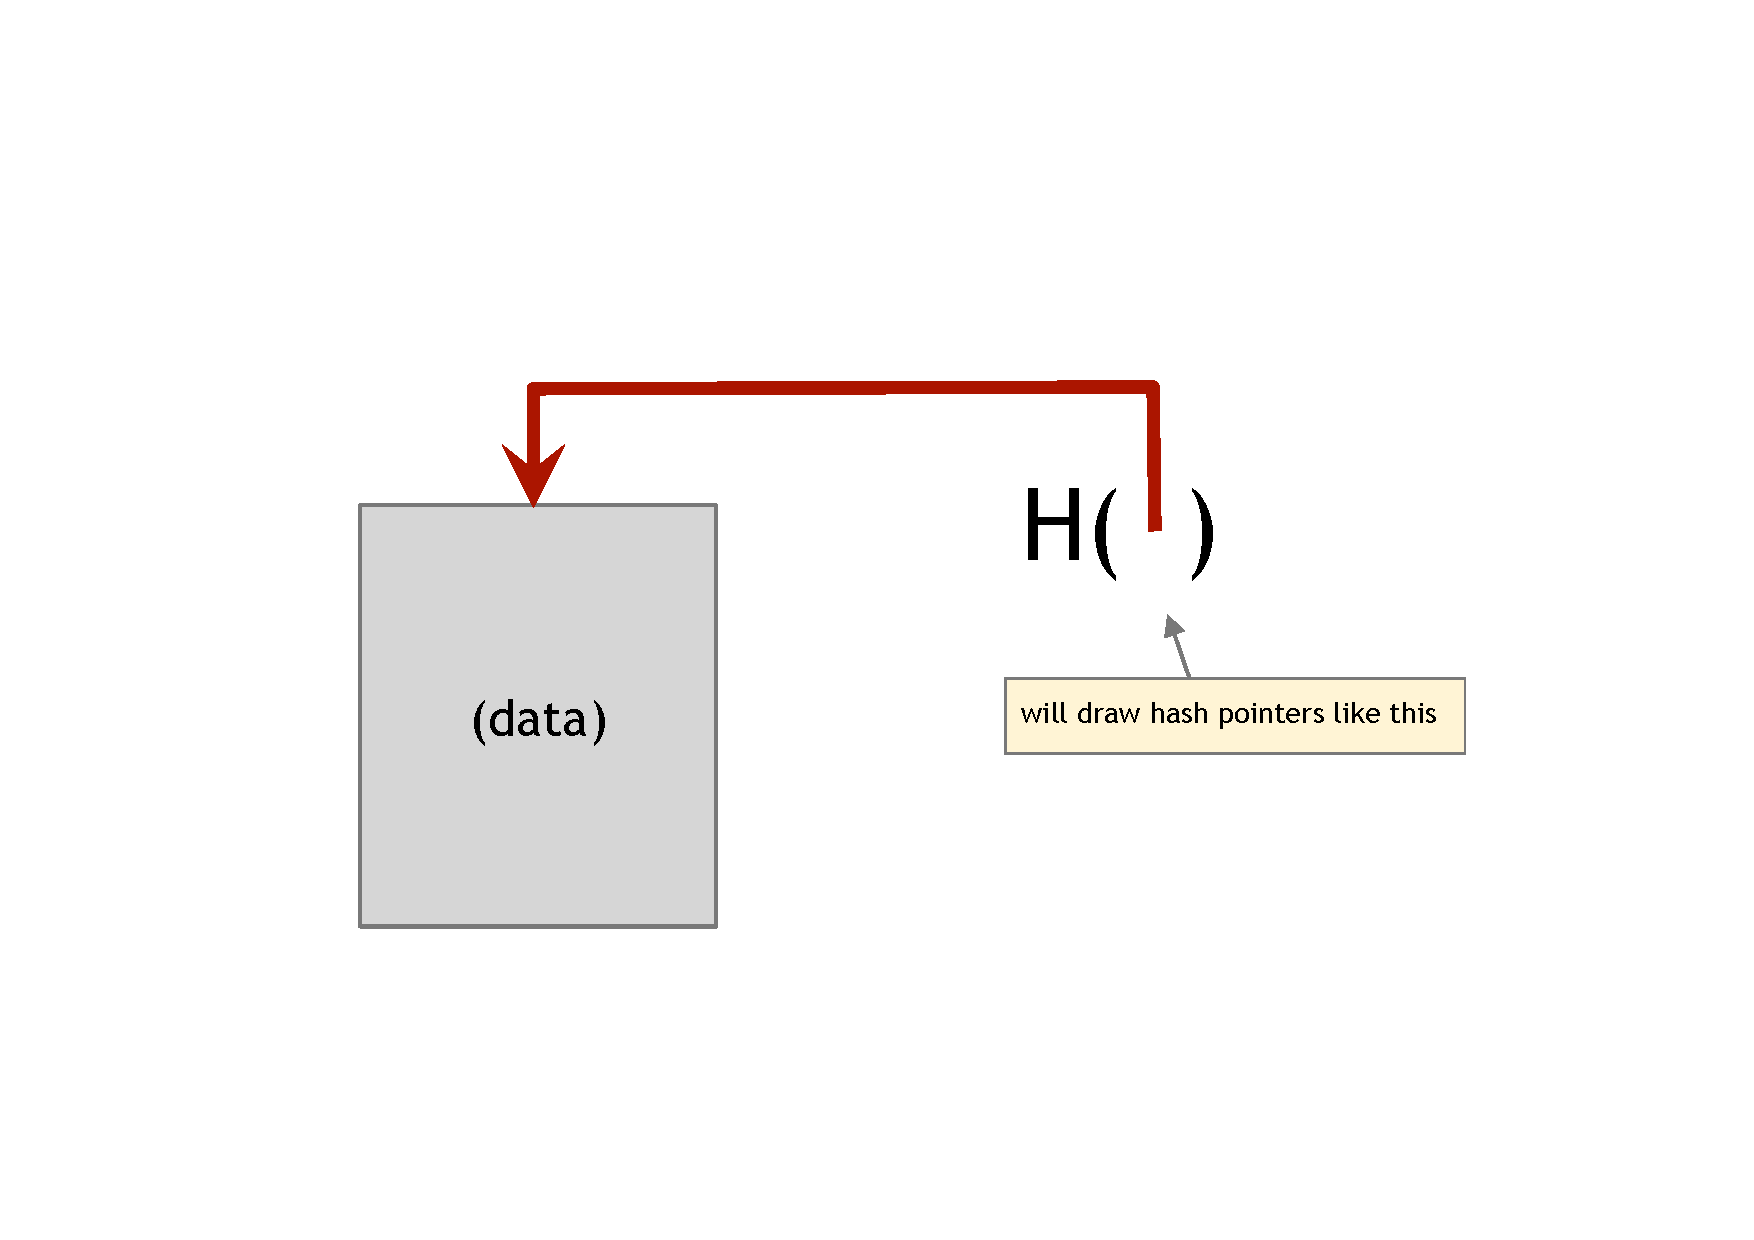
\includegraphics[width=6cm]{hash-pointer}	
\end{center}
\end{column}	
\end{columns}	
	
\end{frame}

%-------------------------------------------------------------------------
\begin{frame}{Blockchain}

\BB{Linked list with hash pointers (\alert{Blockchain})}

\begin{overprint}
\onslide<1|handout:0>
\begin{center}
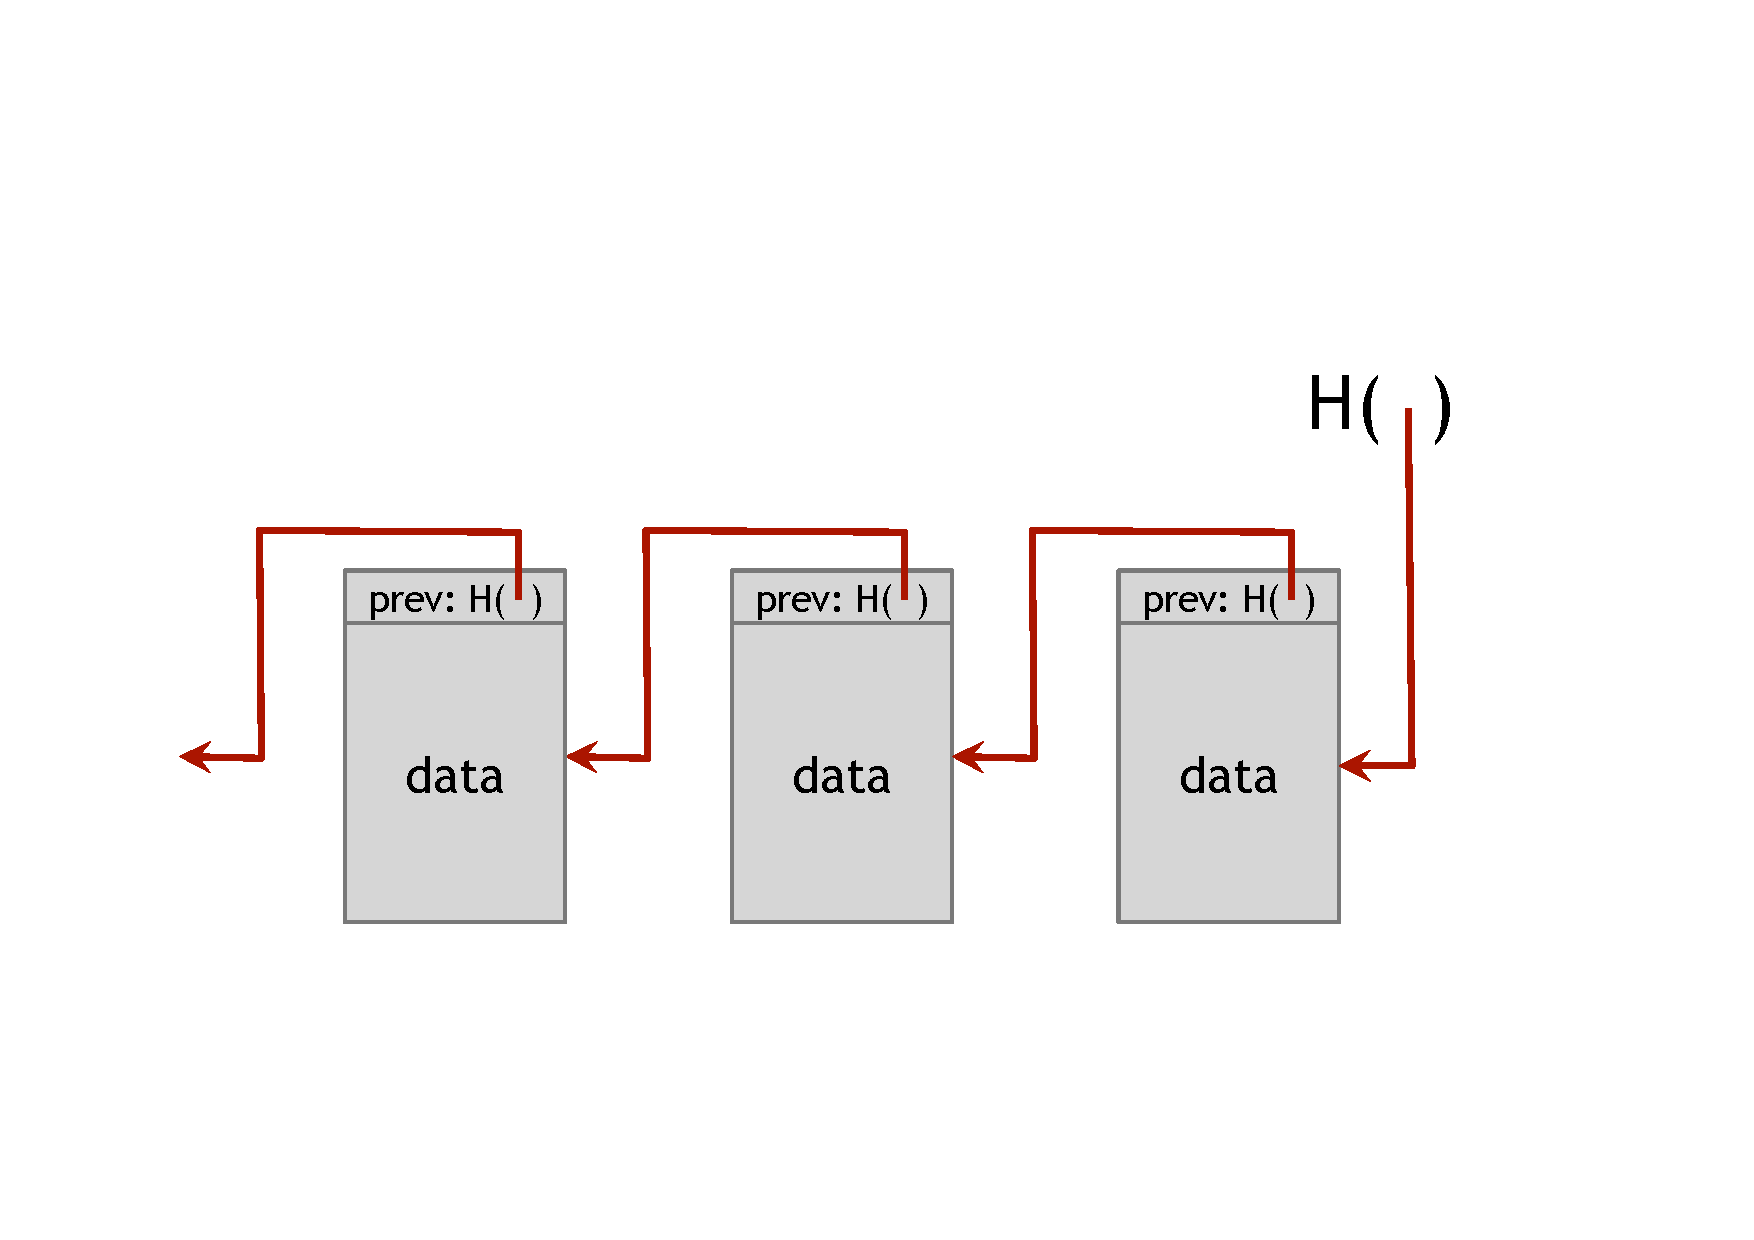
\includegraphics[width=\textwidth,page=1]{blockchain}
\end{center}
\onslide<2|handout:0>
\begin{center}
\includegraphics[width=\textwidth,page=2]{blockchain}
\end{center}
\onslide<3|handout:0>
\begin{center}
\includegraphics[width=\textwidth,page=3]{blockchain}
\end{center}
\onslide<4|handout:1>
\begin{center}
\includegraphics[width=\textwidth,page=4]{blockchain}
\end{center}
\end{overprint}
	

\end{frame}

%-------------------------------------------------------------------------
\begin{frame}{Merkle tree}

\BB{Binary tree with hash pointers  (\alert{Merkle tree})}

\begin{overprint}
\onslide<1|handout:0>
\begin{center}
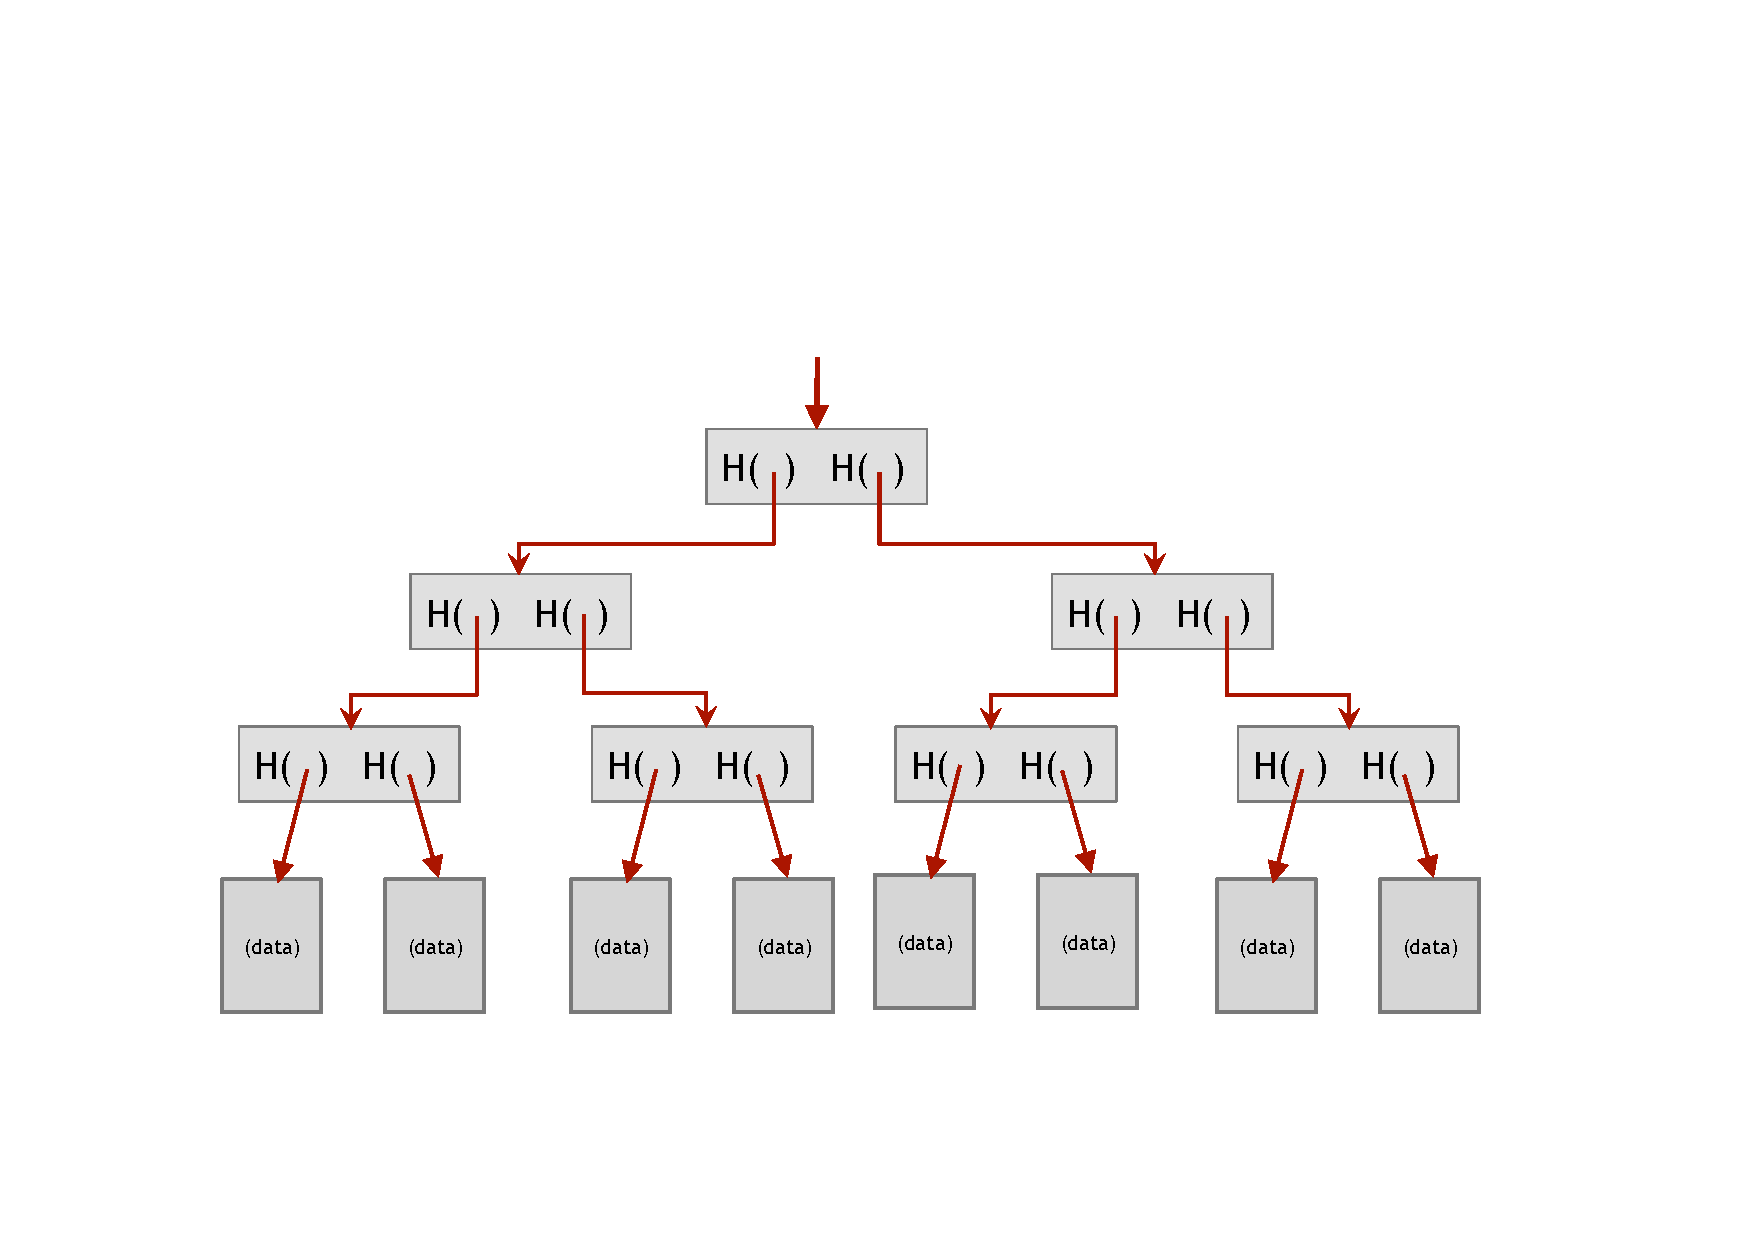
\includegraphics[width=\textwidth,page=1]{merkle-tree}
\end{center}
\onslide<2|handout:1>
\begin{center}
\includegraphics[width=\textwidth,page=2]{merkle-tree}
\end{center}
\end{overprint}
	
\end{frame}

%-------------------------------------------------------------------------
\begin{frame}{Merkle tree}

\BB{Advantages of Merkle Tree}

\BIL	
\item Tree holds many items, but just need to remember the root hash
\item Can verify membership in $O(\log n)$ time/space
\item Variant: sorted Merkle tree
  \BI
	\item Can verify non-membership in $O(\log n)$
	\EI
\EIL
	
\end{frame}

%-------------------------------------------------------------------------
\begin{frame}{Public/private signatures}

\BB{Objectives}

\BIL
\item Only you can sign, but anyone can verify
\item Signature is tied to a particular document\\
			Can't be cut-and-pasted to another doc
\EIL

\BB{API for digital signatures}

\BIL
\item $(\mathit{sk}, \mathit{pk}) \gets \textsf{generateKeys}(\mathit{keysize})$
	\BI
	\item $\mathit{sk}$: secret signing key
	\item	$\mathit{pk}$: public verification key
	\EI
\item  $\mathit{sig} \gets \textsf{sign}(\mathit{sk}, \mathit{message})$
\item  $\mathit{isValid} \gets \textsf{verify}(\mathit{pk}, \mathit{message}, \mathit{sig})$
\EIL

\end{frame}

\subsection{Signatures}

%-------------------------------------------------------------------------
\begin{frame}{Public/private signatures}
	
\BB{Requirements}

\BIL
\item Valid signatures verify:
  \BI
	\item $\textsf{verify}(\mathit{pk}, \mathit{message}, \textsf{sign}(\mathit{sk}, \mathit{message})) = \TRUE$
	\EI
\item An adversary who:
	\BI
	\item knows $\mathit{pk}$
	\item	gets to see signatures on messages of his choice
	\EI
	can't produce a verifiable signature on another message
\EIL

\BB{Bitcoin}
\BI
\item Uses ECDSA (Elliptic Curve Digital Signature Algorithm)
\EI

\end{frame}

%-------------------------------------------------------------------------
\begin{frame}{Public/private signatures}	

\BB{Public keys $\equiv$ identity}
\BI
\item If you see $\mathit{sig}$ such that $\textsf{verify}(\mathit{pk}, \mathit{msg}, \mathit{sig})=\TRUE$, think of it as “$\mathit{pk}$ says [$\mathit{msg}]$”
\EI

\BB{Decentralized identity management}

\BI
\item Anybody can make a new identity at any time
\item No central point of coordination
\item These identities are called “addresses” in Bitcoin
\EI

\BB{Privacy}
\BI
\item Addresses not directly connected to real-world identity.
\item But observer can link together an address's activity over time, make inferences
\EI

\end{frame}

\section{Naive coins}
\subsection{Goofy coin}

%-------------------------------------------------------------------------
\begin{frame}{GoofyCoin}

\begin{overprint}
\onslide<1|handout:0>
\begin{center}

\includegraphics[width=\textwidth,page=1]{goofy-coin}
\end{center}
\onslide<2|handout:0>
\begin{center}

\includegraphics[width=\textwidth,page=2]{goofy-coin}
\end{center}
\onslide<3|handout:0>
\begin{center}

\includegraphics[width=\textwidth,page=3]{goofy-coin}
\end{center}
\onslide<4|handout:0>
\begin{center}

\includegraphics[width=\textwidth,page=4]{goofy-coin}
\end{center}
\onslide<5|handout:1>
\begin{center}

\includegraphics[width=\textwidth,page=5]{goofy-coin}
\end{center}
\end{overprint}
	
\end{frame}

\subsection{ScroogeCoin}

%-------------------------------------------------------------------------
\begin{frame}{ScroogeCoin}

\begin{overprint}
\onslide<1|handout:0>
\begin{center}

\includegraphics[width=\textwidth,page=1]{scrooge-coin}
\end{center}
\onslide<2|handout:0>
\begin{center}

\includegraphics[width=\textwidth,page=2]{scrooge-coin}
\end{center}
\onslide<3|handout:0>
\begin{center}

\includegraphics[width=\textwidth,page=3]{scrooge-coin}
\end{center}
\onslide<4|handout:0>
\begin{center}

\includegraphics[width=\textwidth,page=4]{scrooge-coin}
\end{center}
\onslide<5|handout:1>
\begin{center}

\includegraphics[width=\textwidth,page=5]{scrooge-coin}
\end{center}
\end{overprint}

\end{frame}

\section{Bitcoin Basics}

\begin{frame}{Definitions}
\begin{definition}[Transaction]
	A transaction is a transfer of Bitcoin value that is broadcast to the network and collected into blocks.
\end{definition}

\BI
\item  A transaction typically references previous transaction outputs as new transaction inputs and dedicates all input Bitcoin values to new outputs.
\item Transactions are not encrypted, so it is possible to browse and view every transaction ever collected into a block.
\EI

\end{frame}


%%%%%%%%%%%%%%%%%%%%%%%%%%%%%%%%%%%%%%%%%%%%%%%%%%%%%%%%%%%%%%%%%%%%%%%%%%
\subsection{Ledger}
%%%%%%%%%%%%%%%%%%%%%%%%%%%%%%%%%%%%%%%%%%%%%%%%%%%%%%%%%%%%%%%%%%%%%%%%%%

%-------------------------------------------------------------------------

\begin{frame}{Blocks}
	
\begin{columns}
\begin{column}{0.5\textwidth}
\BB{Transaction data is bundled together and recorded in files called blocks}
\BI
\item Single unit of work for miners
\item Limit length of hash-chain of blocks
\item Faster to verify history
\EI
\end{column}
\begin{column}{0.5\textwidth}
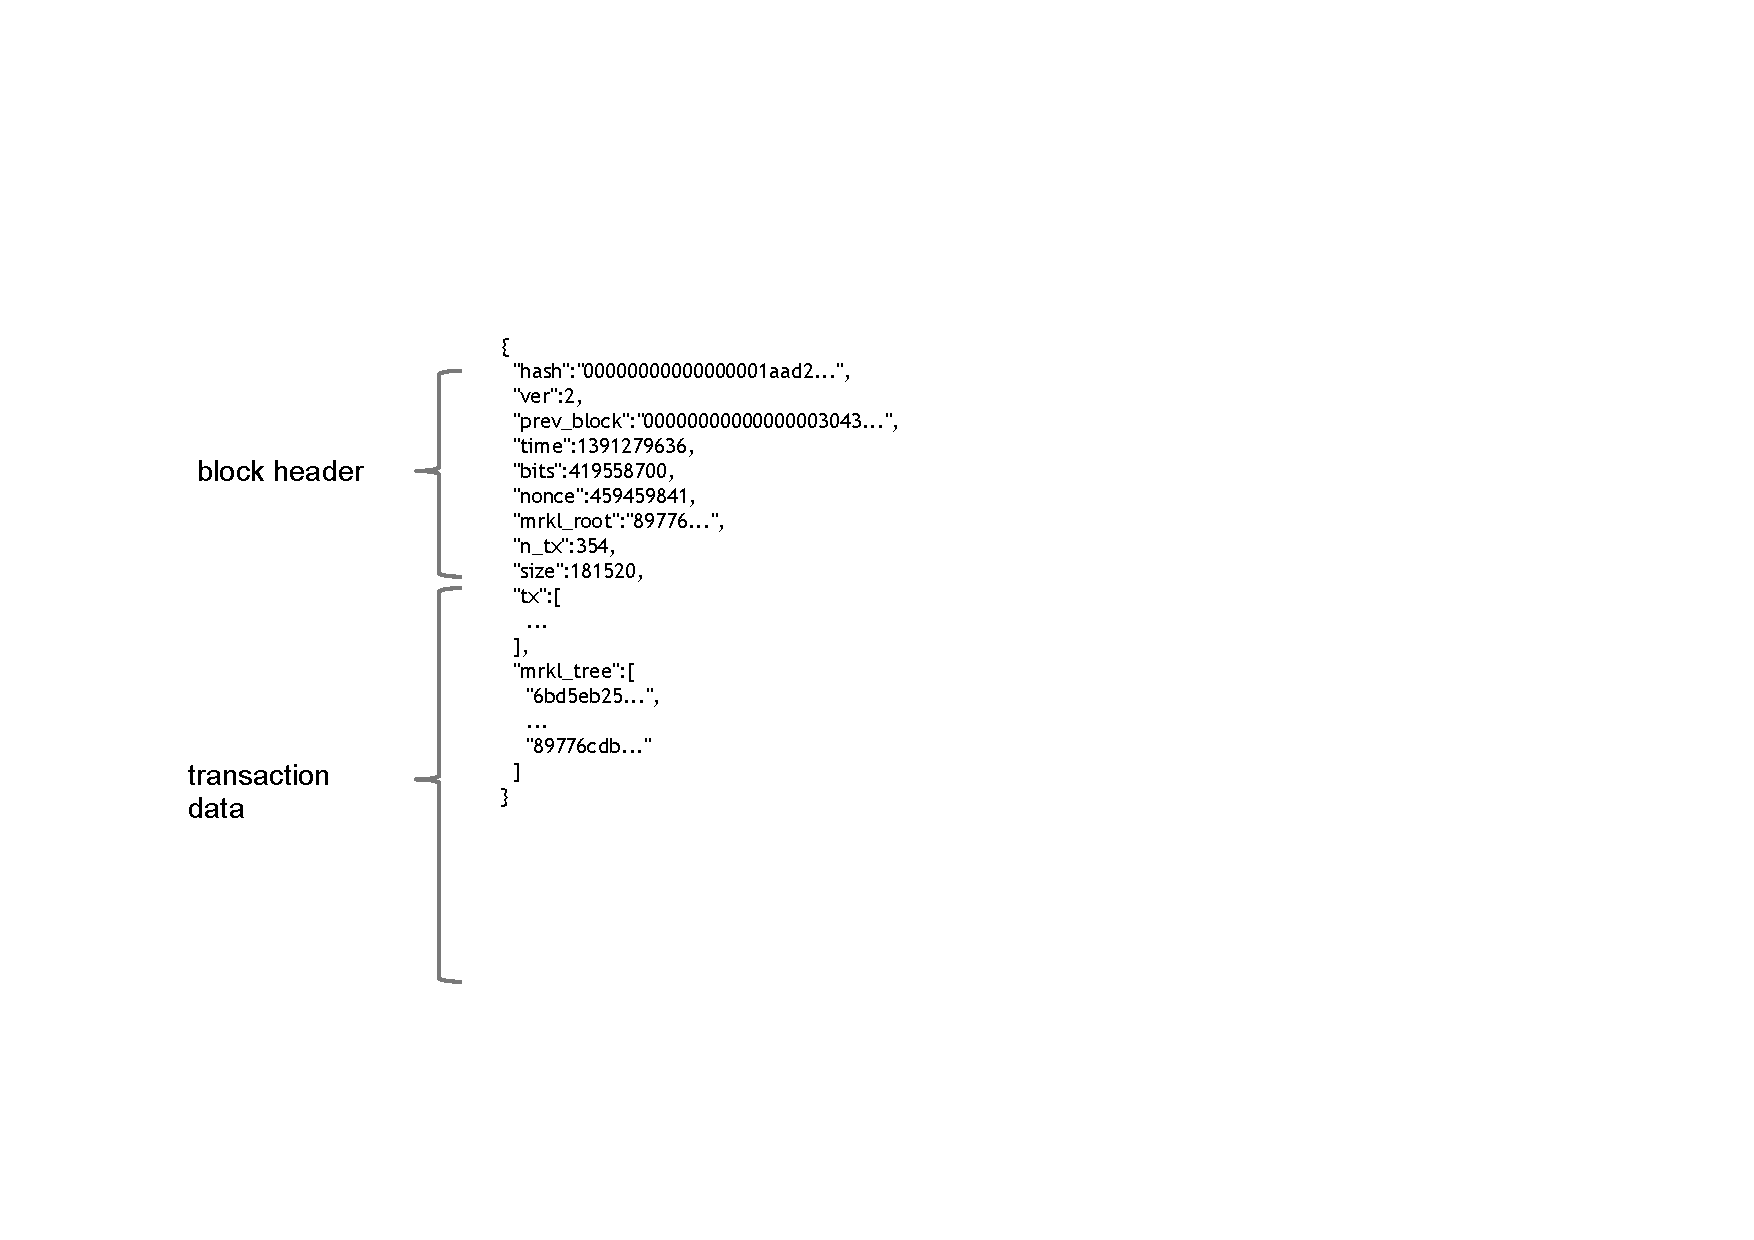
\includegraphics[width=\textwidth]{block}
\end{column}
\end{columns}


\end{frame}

%-------------------------------------------------------------------------

\begin{frame}{Structure of the blockchain}
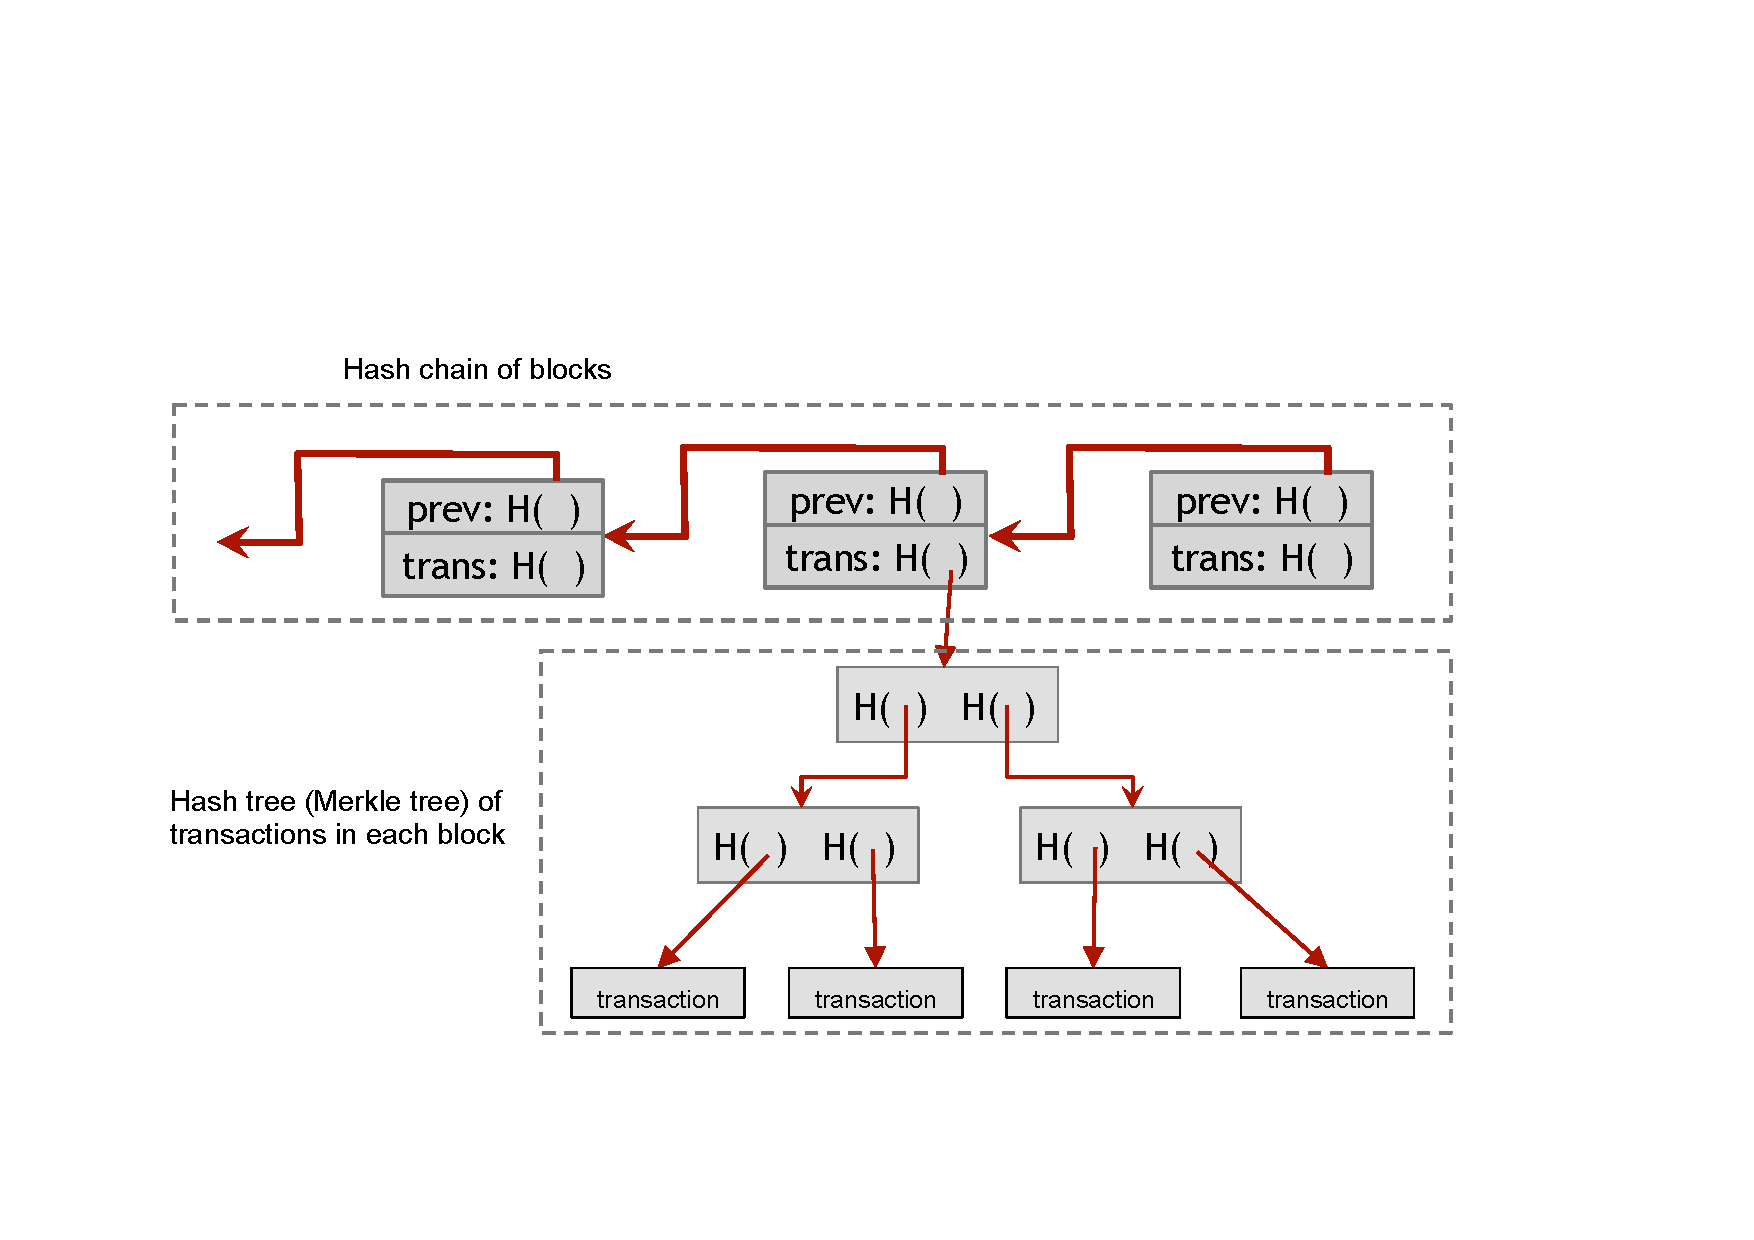
\includegraphics[width=\textwidth]{blockchain-actual}
\end{frame}

%-------------------------------------------------------------------------

\begin{frame}{Blockchain size}
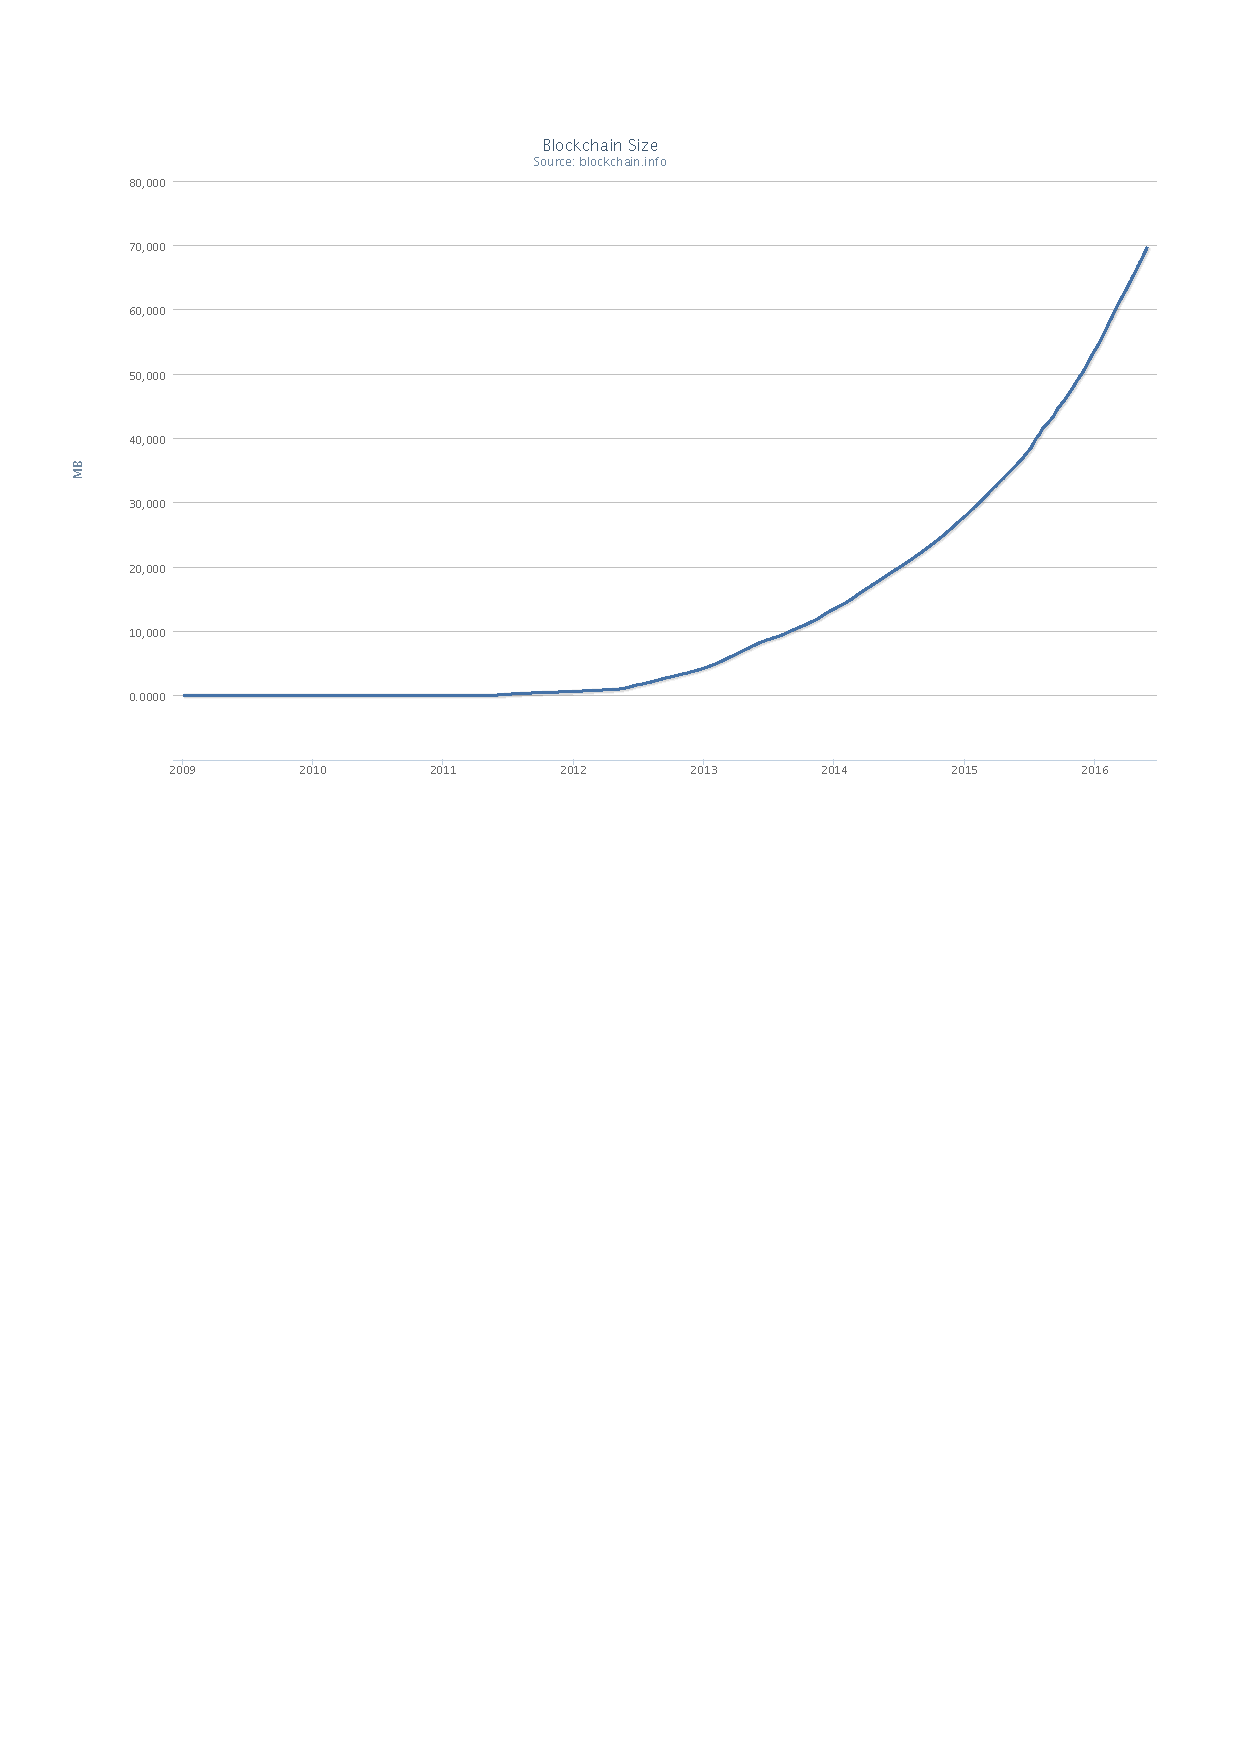
\includegraphics[width=\textwidth]{blockchain-size}
\end{frame}

%-------------------------------------------------------------------------
\begin{frame}{An account-based ledger (not Bitcoin)}
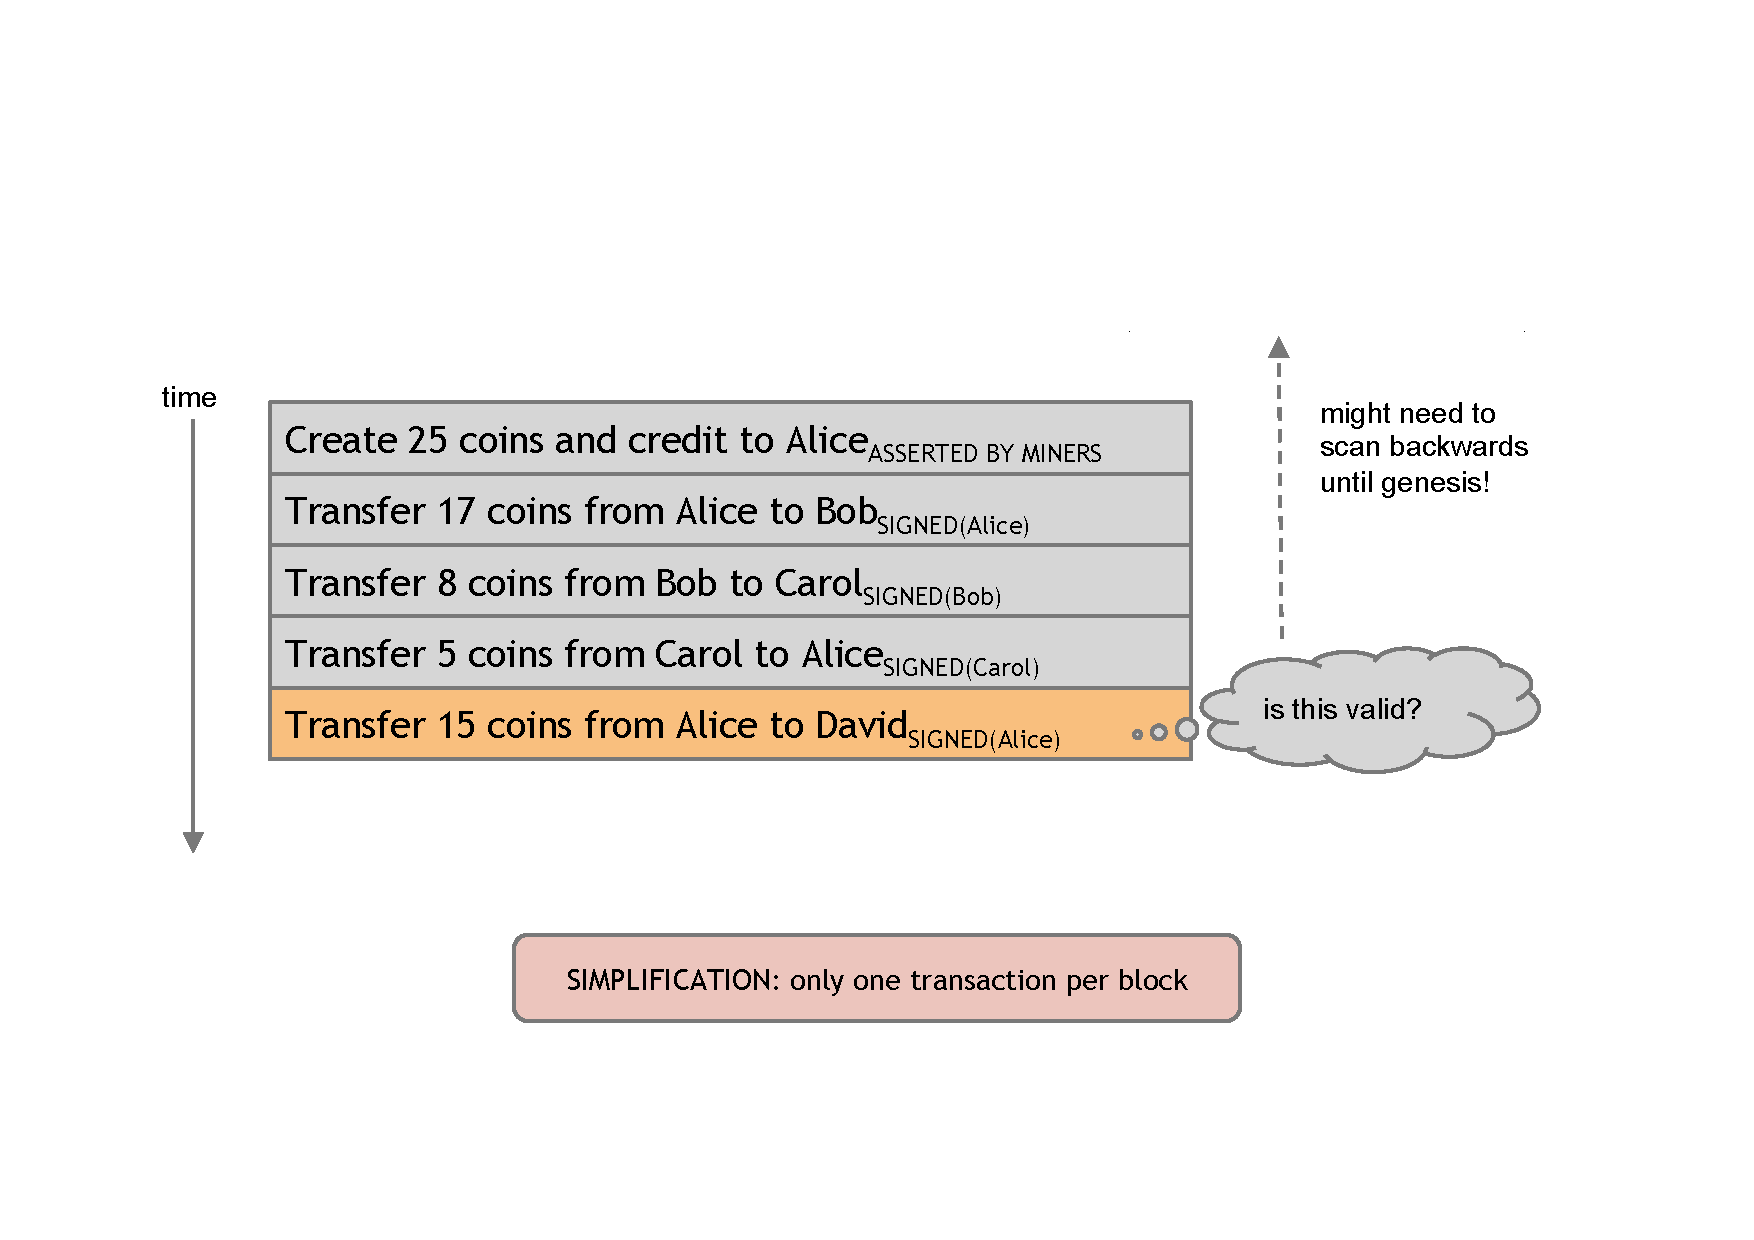
\includegraphics[width=\textwidth,page=1]{ledger}
\end{frame}

%-------------------------------------------------------------------------
\begin{frame}{A transaction-based ledger (Bitcoin)}
\includegraphics[width=\textwidth,page=2]{ledger}
\end{frame}

%-------------------------------------------------------------------------
\begin{frame}{Merging value}
\includegraphics[width=\textwidth,page=3]{ledger}
\end{frame}

%-------------------------------------------------------------------------
\begin{frame}{Joint payments}
\includegraphics[width=\textwidth,page=4]{ledger}
\end{frame}


%%%%%%%%%%%%%%%%%%%%%%%%%%%%%%%%%%%%%%%%%%%%%%%%%%%%%%%%%%%%%%%%%%%%%%%%%%
\section{Decentralization in Bitcoin}
%%%%%%%%%%%%%%%%%%%%%%%%%%%%%%%%%%%%%%%%%%%%%%%%%%%%%%%%%%%%%%%%%%%%%%%%%%

\begin{frame}{Aspects of decentralization in Bitcoin}

\BB{Technological aspects of decentralization in Bitcoin}
\BI
\item Who maintains the ledger?
\item Who has authority over which transactions are valid?
\item Who creates new Bitcoins?
\EI

\BB{Socio-economical aspects of decentralization in Bitcoin}
\BI
\item Who determines how the rules of the system change?
\item Who maintains the software
\item How do Bitcoins acquire exchange value?
\EI

\BB{Beyond the protocol}
\BI
\item exchanges, wallet software, service providers...
\EI

\end{frame}

%-------------------------------------------------------------------------
\begin{frame}{Decentralization in Bitcoin}


\BB{Peer-to-peer network}
\BI
\item	Open to anyone, low barrier to entry
\EI

\BB{Consensus}
\BI
\item	Consensus is reached by waiting long enough to observe confirmations 
from most of the network
\EI

\BB{Mining}
\BI
\item Open to anyone, but inevitable concentration of power
	often seen as undesirable
\EI

\end{frame}

\subsection{BitCoin P2P Network}


%-------------------------------------------------------------------------
\begin{frame}{Bitcoin is a peer-to-peer system}
	
\BB{
When Alice wants to pay Bob,\\ she broadcasts the transaction to all Bitcoin nodes
}

\begin{center}
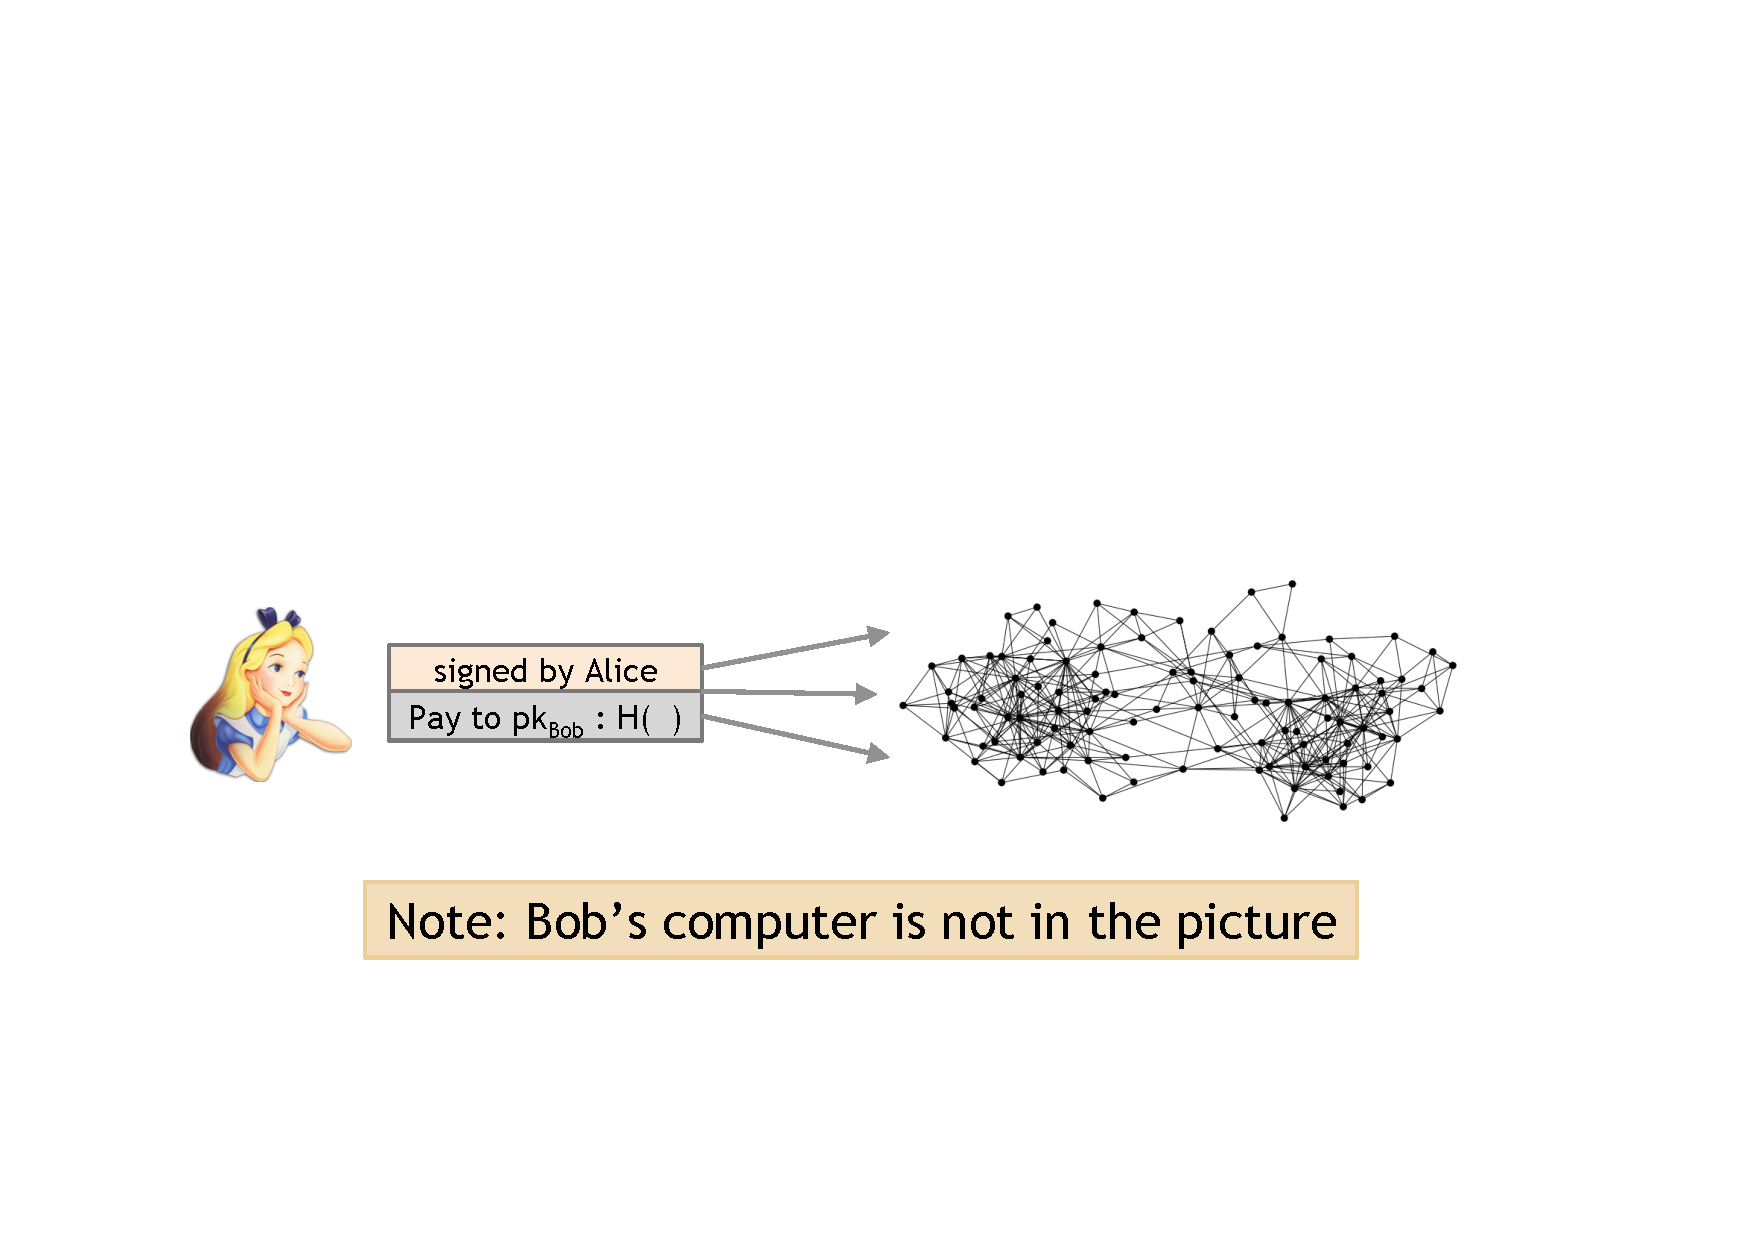
\includegraphics[width=\textwidth]{p2p}
\end{center}

\end{frame}





%-------------------------------------------------------------------------
\begin{frame}{Bitcoin P2P network}
	
\BIL
\item Ad-hoc protocol (runs on TCP port 8333)
\item Ad-hoc network with random topology
\item All nodes are equal
\item New nodes can join at any time
\item Forget non-responding nodes after 3 hr
\EIL	

\end{frame}

%-------------------------------------------------------------------------
\begin{frame}{Bitcoin P2P network}
	
\begin{overprint}
\onslide<1|handout:1>
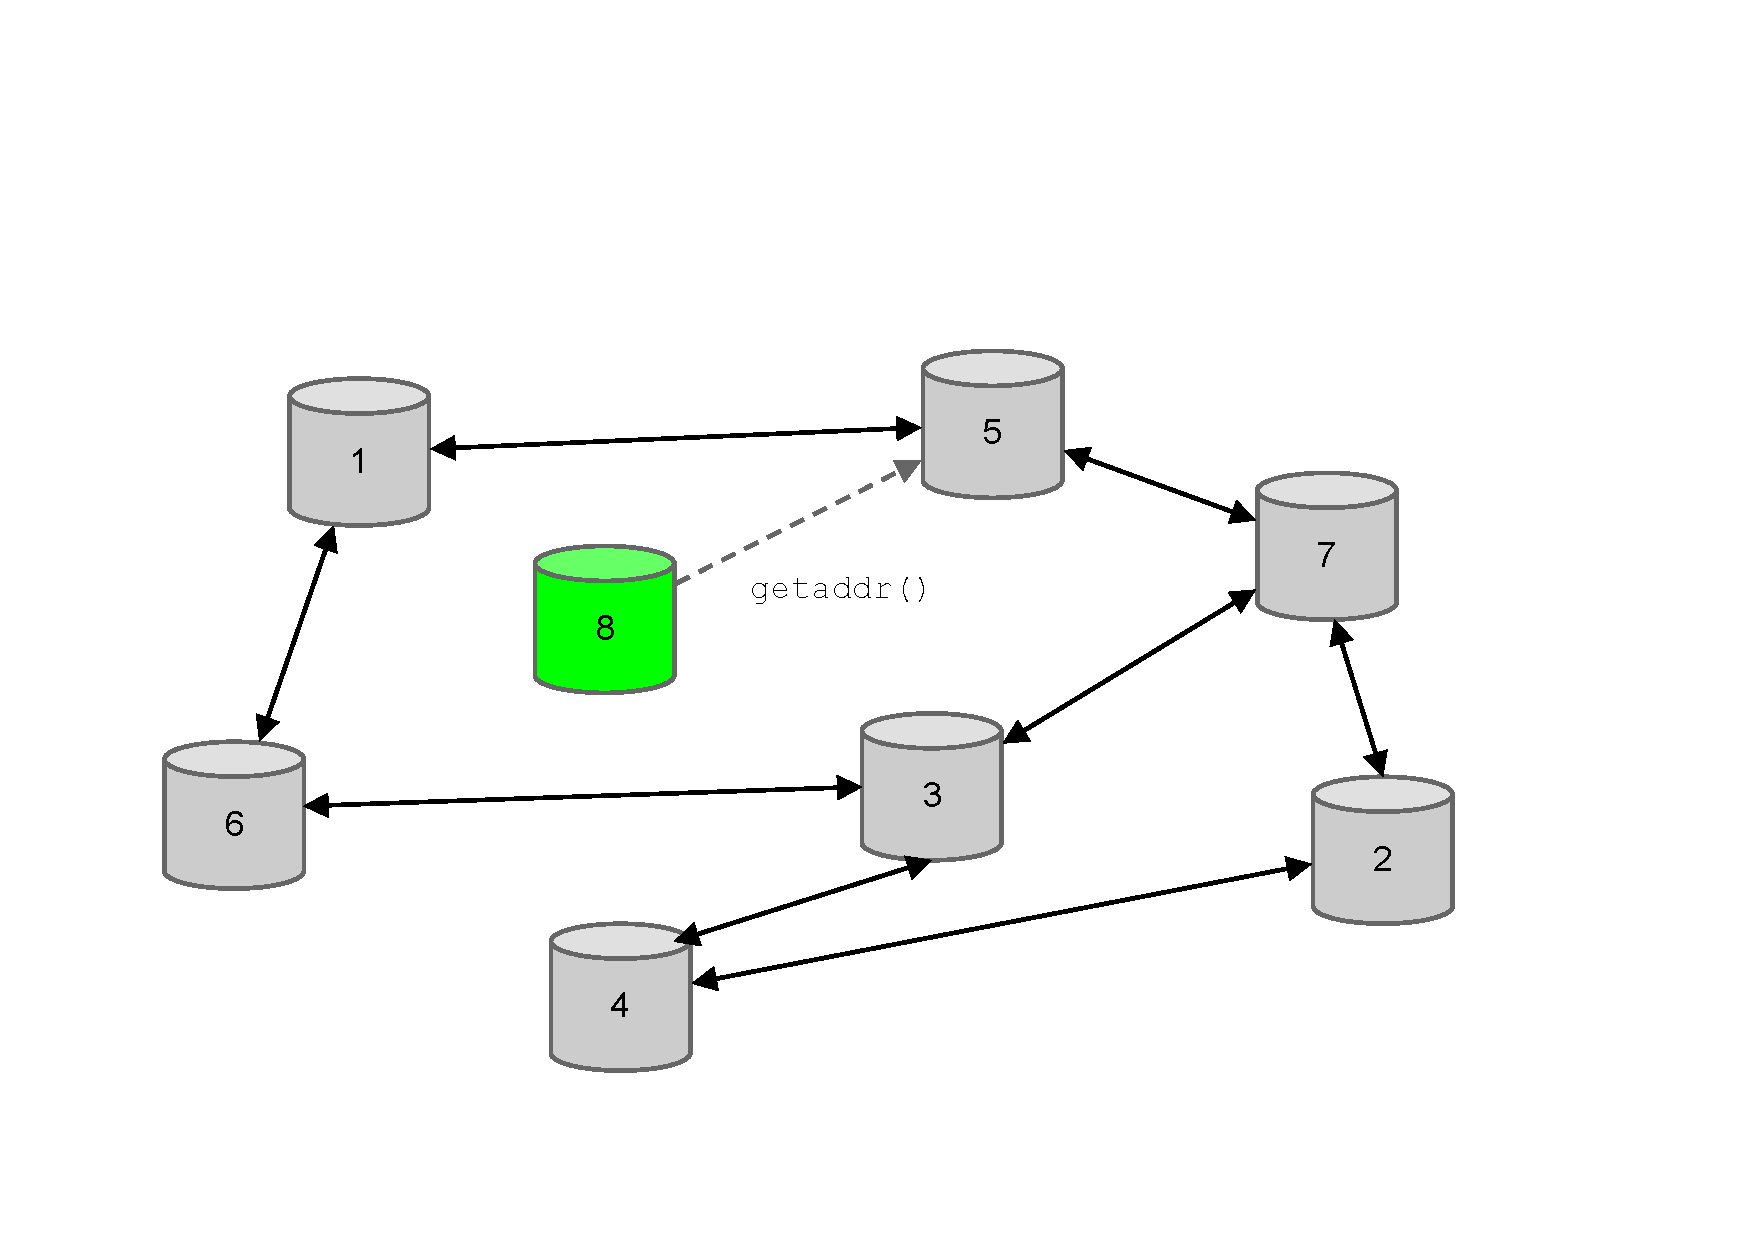
\includegraphics[width=\textwidth,page=1]{p2p-join}
\onslide<2|handout:2>
\includegraphics[width=\textwidth,page=2]{p2p-join}
\onslide<3|handout:3>
\includegraphics[width=\textwidth,page=3]{p2p-join}
\onslide<4|handout:4>
\includegraphics[width=\textwidth,page=4]{p2p-join}
\end{overprint}

\end{frame}

%-------------------------------------------------------------------------
\begin{frame}{Network characteristics}
\BB{How big is the network?}
\BI
\item Impossible to measure exactly
\item Estimates-up to 1M IP addresses/month
\item Only about 5-10k “full nodes”
\EI

\begin{columns}[T]
\begin{column}{0.48\textwidth}
\BB{Full nodes}
\BI
\item Permanently connected
\item Store entire block chain
\item Hear and forward every node/transaction
\item Tracking the Unspent Transaction Output (UTXO)
	\BI
	\item Currently $\approx 38$ M UTXOs
	\item Can easily fit into RAM
	\EI
\EI
\end{column}
\begin{column}{0.48\textwidth}

\BB{Thin clients}

\BI
\item Idea: don’t store everything
\item Store block headers only
\item Request transactions as needed, to verify incoming payment
\item Trust fully-validating nodes
\item 1000x cost savings! 
\EI
\end{column}

\end{columns}

\end{frame}

%-------------------------------------------------------------------------
\begin{frame}{Software diversity}

\BI
\item About 90\% of nodes run “Core Bitcoin” (C++)
	\BI
	\item Some are out of date versions
	\EI
\item Other implementations running successfully
	\BI
	\item \texttt{BitcoinJ} (Java)
	\item \texttt{Libbitcoin} (C++)
	\item \texttt{btcd} (Go)
	\EI
\item “Original Satoshi client”
\EI

\end{frame}


\subsection{Consensus basics}

%-------------------------------------------------------------------------
\begin{frame}{Bitcoin consensus}

\BB{Bitcoin's key challenge}

\BI
\item Key technical challenge of decentralized e-cash: \alert{distributed consensus} 
\item or, how to decentralize ScroogeCoin
\EI

\BB{Theory vs practice}

\BI
\item Remember the theoretical impossibility results
\item Bitcoin consensus works better in practice than in theory
\item Theory is still catching up
\EI
	
\end{frame}





%-------------------------------------------------------------------------
\begin{frame}{How consensus \underline{could} work in BitCoin}
	
At any given time:
\BIL
\item All nodes have a sequence of blocks of transactions they've reached consensus on
\item Each node has a set of outstanding transactions it has heard about 
\EIL

\begin{center}
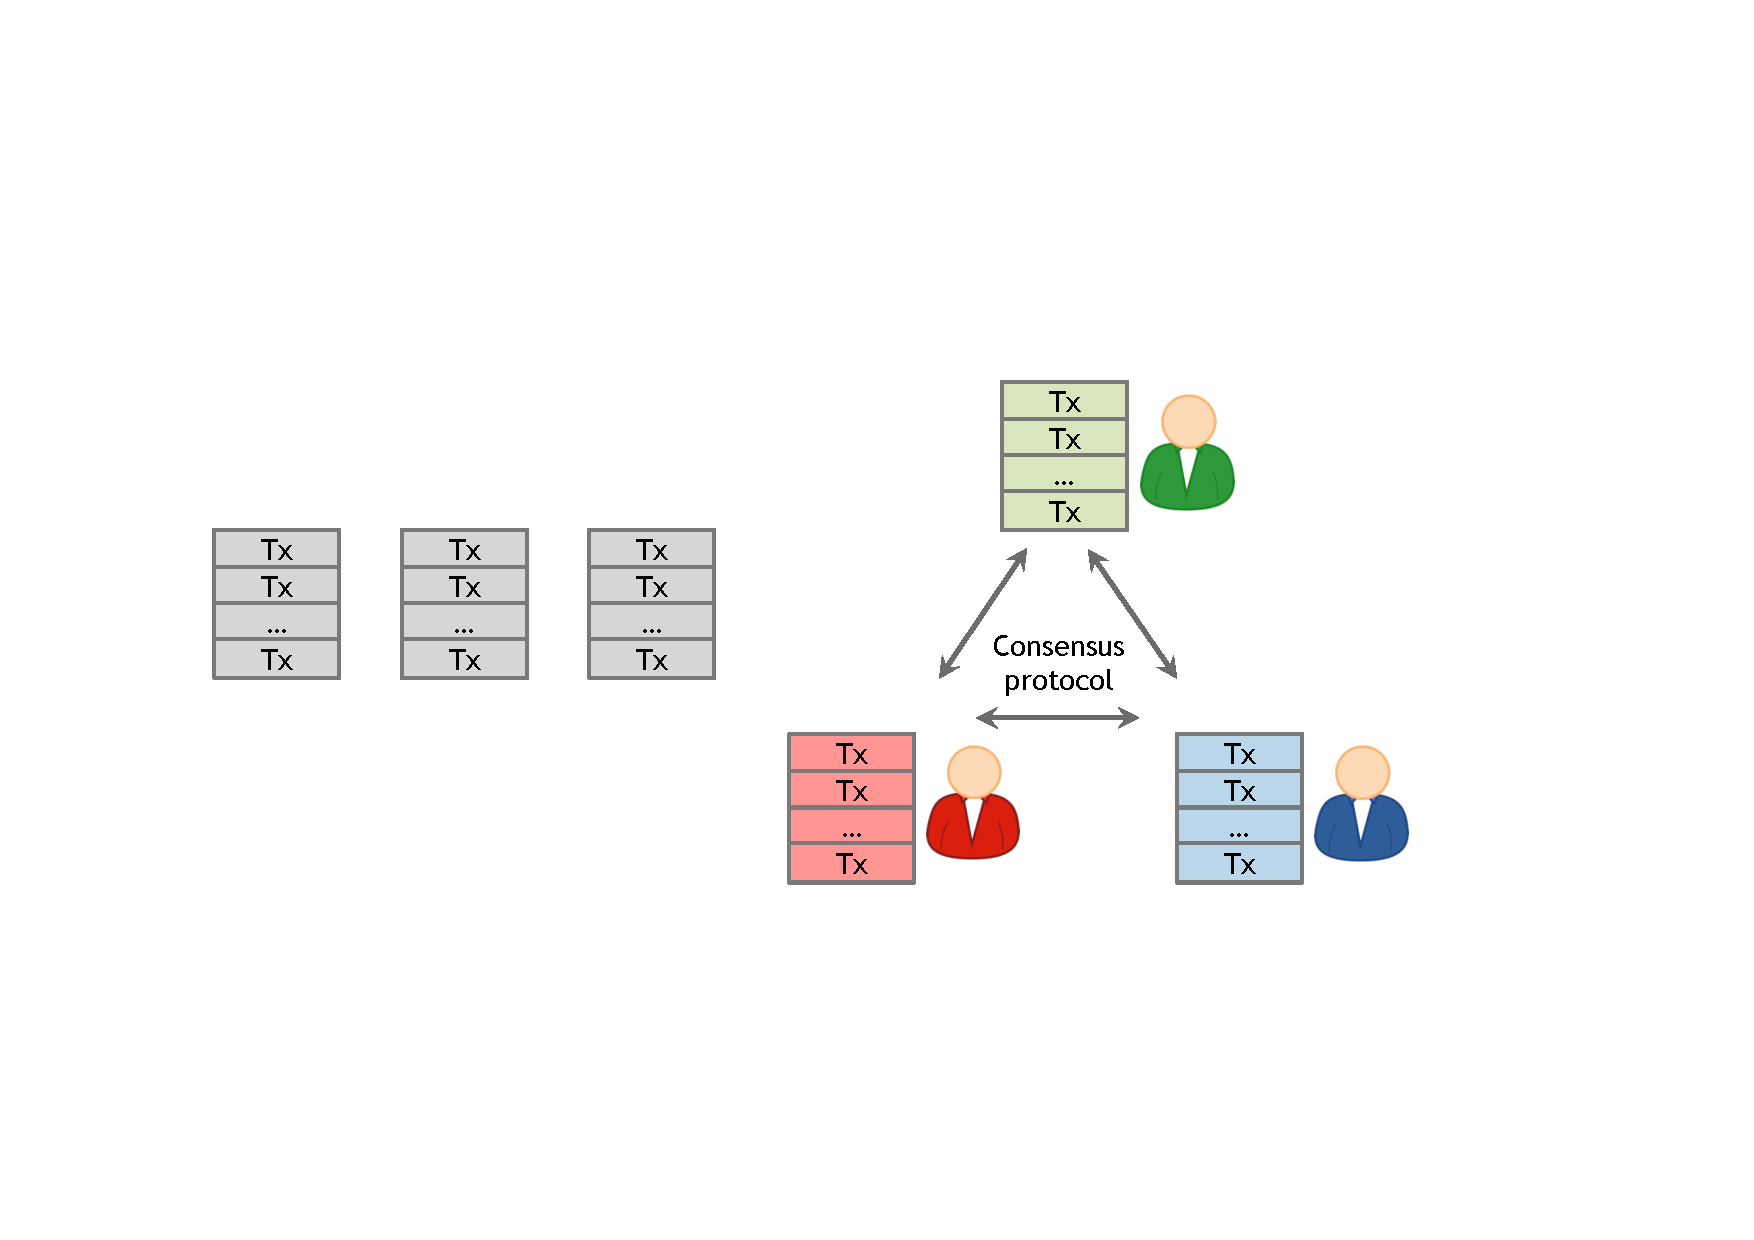
\includegraphics[width=0.8\textwidth]{consensus-could}
\end{center}

\end{frame}


%-------------------------------------------------------------------------
\begin{frame}{Consensus without identity}
\BB{Why identity?}
\BI
\item Pragmatic: some protocols need node IDs
\item Security: assume less than 50\% are malicious
\EI

\BB{Why don't Bitcoin nodes have identities?}
\BI
\item Identity is hard in a P2P system — Sybil attack
\item Pseudo-anymity is a goal of Bitcoin
\EI



\end{frame}

%-------------------------------------------------------------------------
\begin{frame}{Key idea: implicit consensus}
\BIL
\item New transactions are sent to all nodes
\item Each node collects new transactions into a block
\item In each round a random node gets to broadcast its block
\item This node proposes the next block in the chain
\item Other nodes implicitly accept/reject this block
	\BI
	\item by either extending it 
	\item or ignoring it and extending chain from earlier block
	\EI
\item Every block contains hash of the block it extends
\EI


\end{frame}


%-------------------------------------------------------------------------
\begin{frame}{What can a malicious node do?}

Honest nodes will extend the longest valid branch

\begin{center}
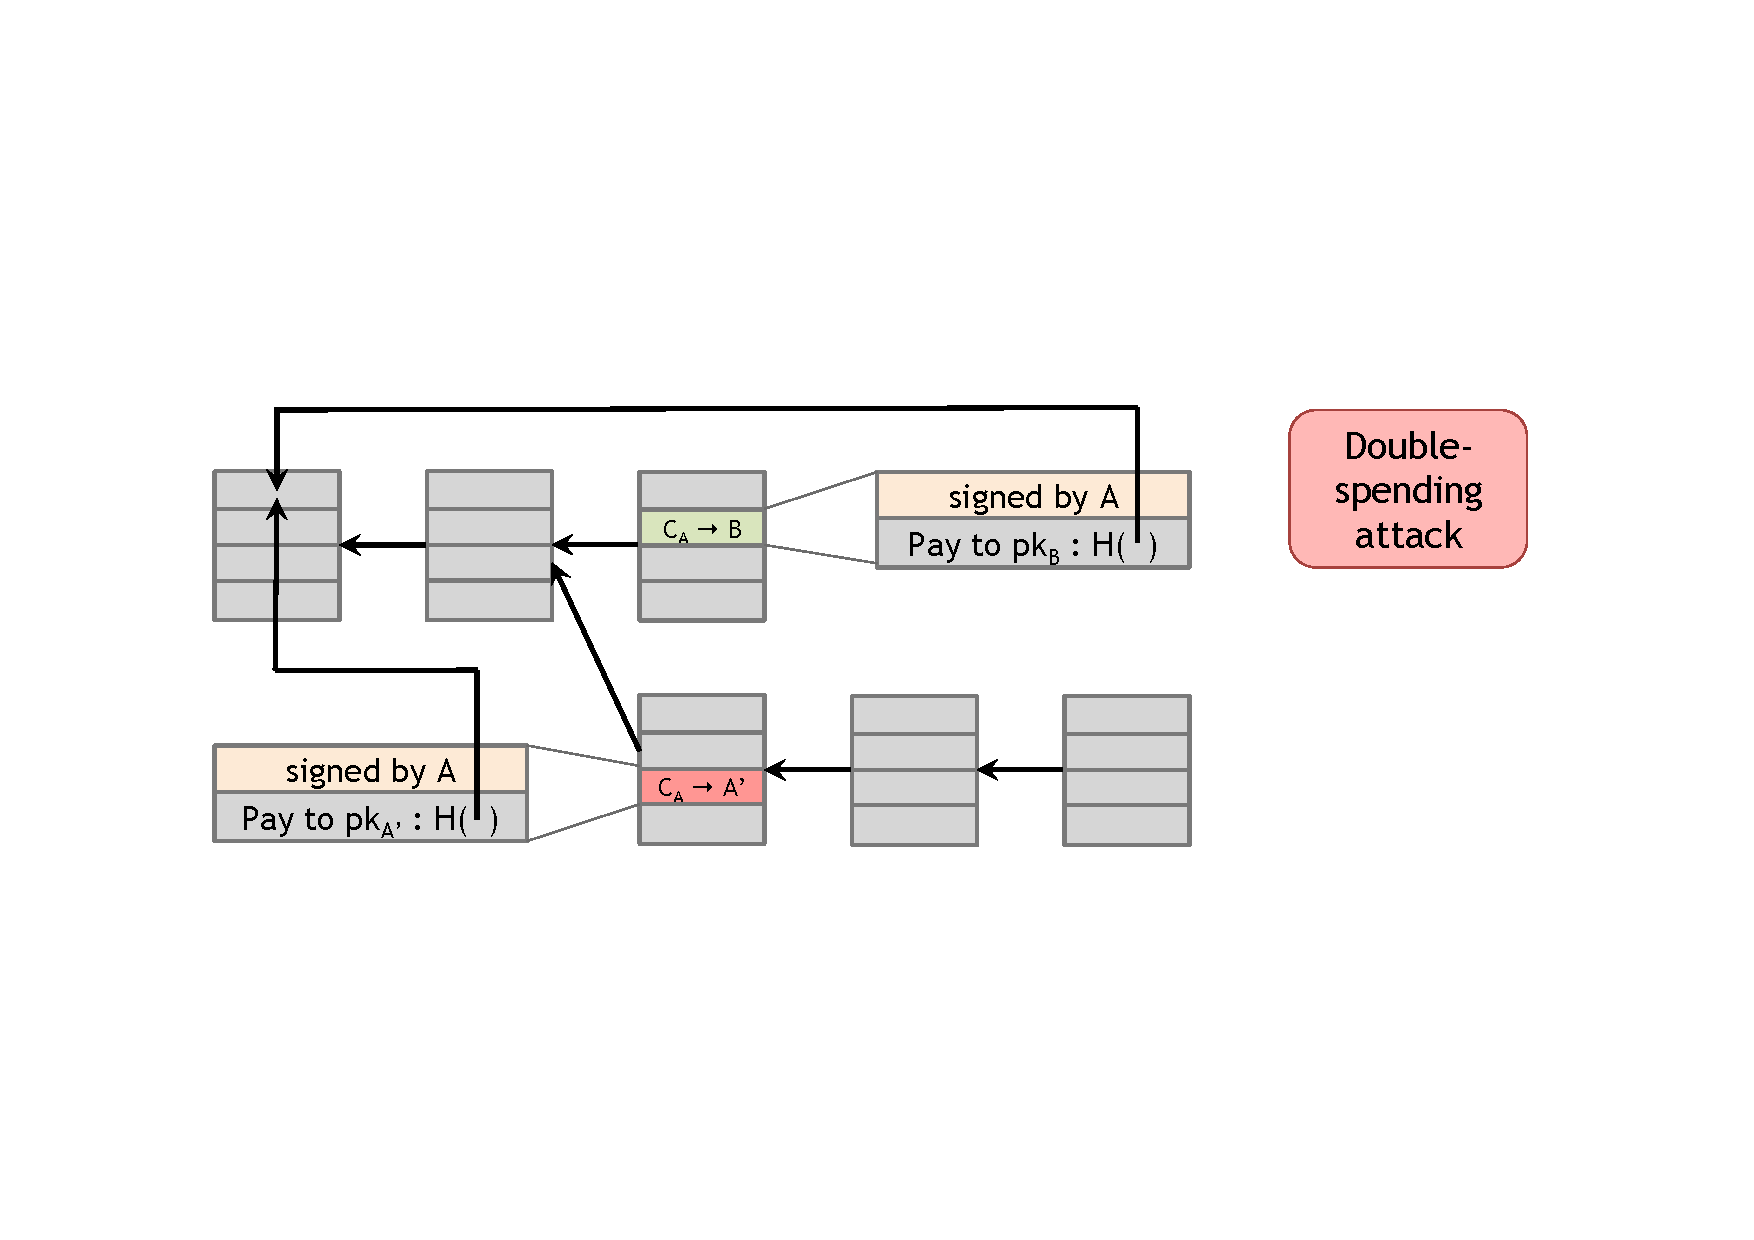
\includegraphics[width=\textwidth]{double1}
\end{center}


\end{frame}

%-------------------------------------------------------------------------
\begin{frame}{What can a malicious node do?}

From Bob the merchant's point of view

\begin{center}
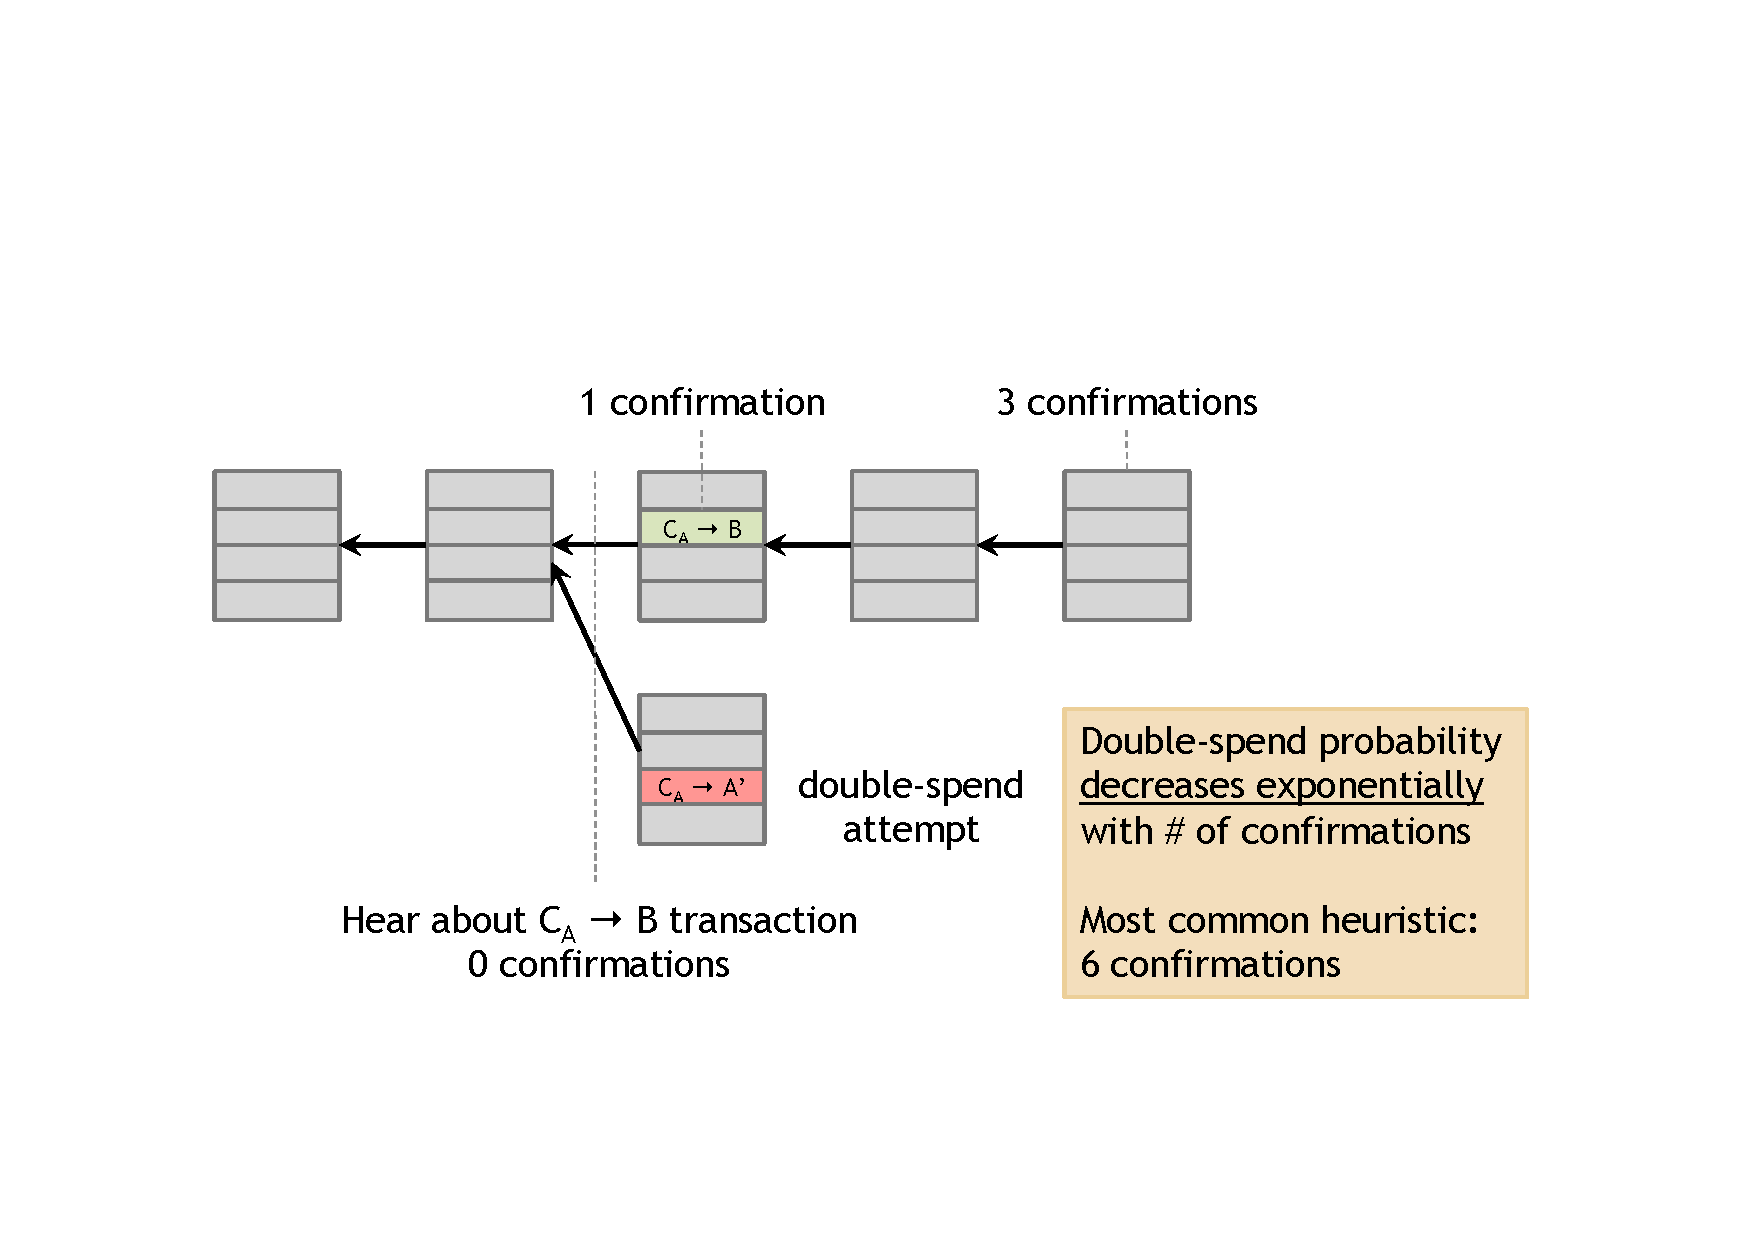
\includegraphics[width=\textwidth]{double2}
\end{center}


\end{frame}

%-------------------------------------------------------------------------
\begin{frame}{Recap}

\BIL
\item Protection against invalid transactions is cryptographic, but enforced by consensus

\item Protection against double-spending is purely by consensus

\item You're never 100\% sure a transaction is in consensus branch. Guarantee is probabilistic
\EIL


\end{frame}

%%%%%%%%%%%%%%%%%%%%%%%%%%%%%%%%%
\subsection{Mining}
%%%%%%%%%%%%%%%%%%%%%%%%%%%%%%%%%

%-------------------------------------------------------------------------
\begin{frame}{Some things Bitcoin does differently}
	
\BB{Introduces incentives}
\BI
\item Possible only because it's a currency!
\EI

\BB{Embraces randomness}
\BI
\item Does away with the notion of a specific end-point
\item Consensus happens over long time scales — about 1 hour
\EI

\end{frame}



%-------------------------------------------------------------------------
\begin{frame}{Incentives for behaving honestly -- Block reward}
	
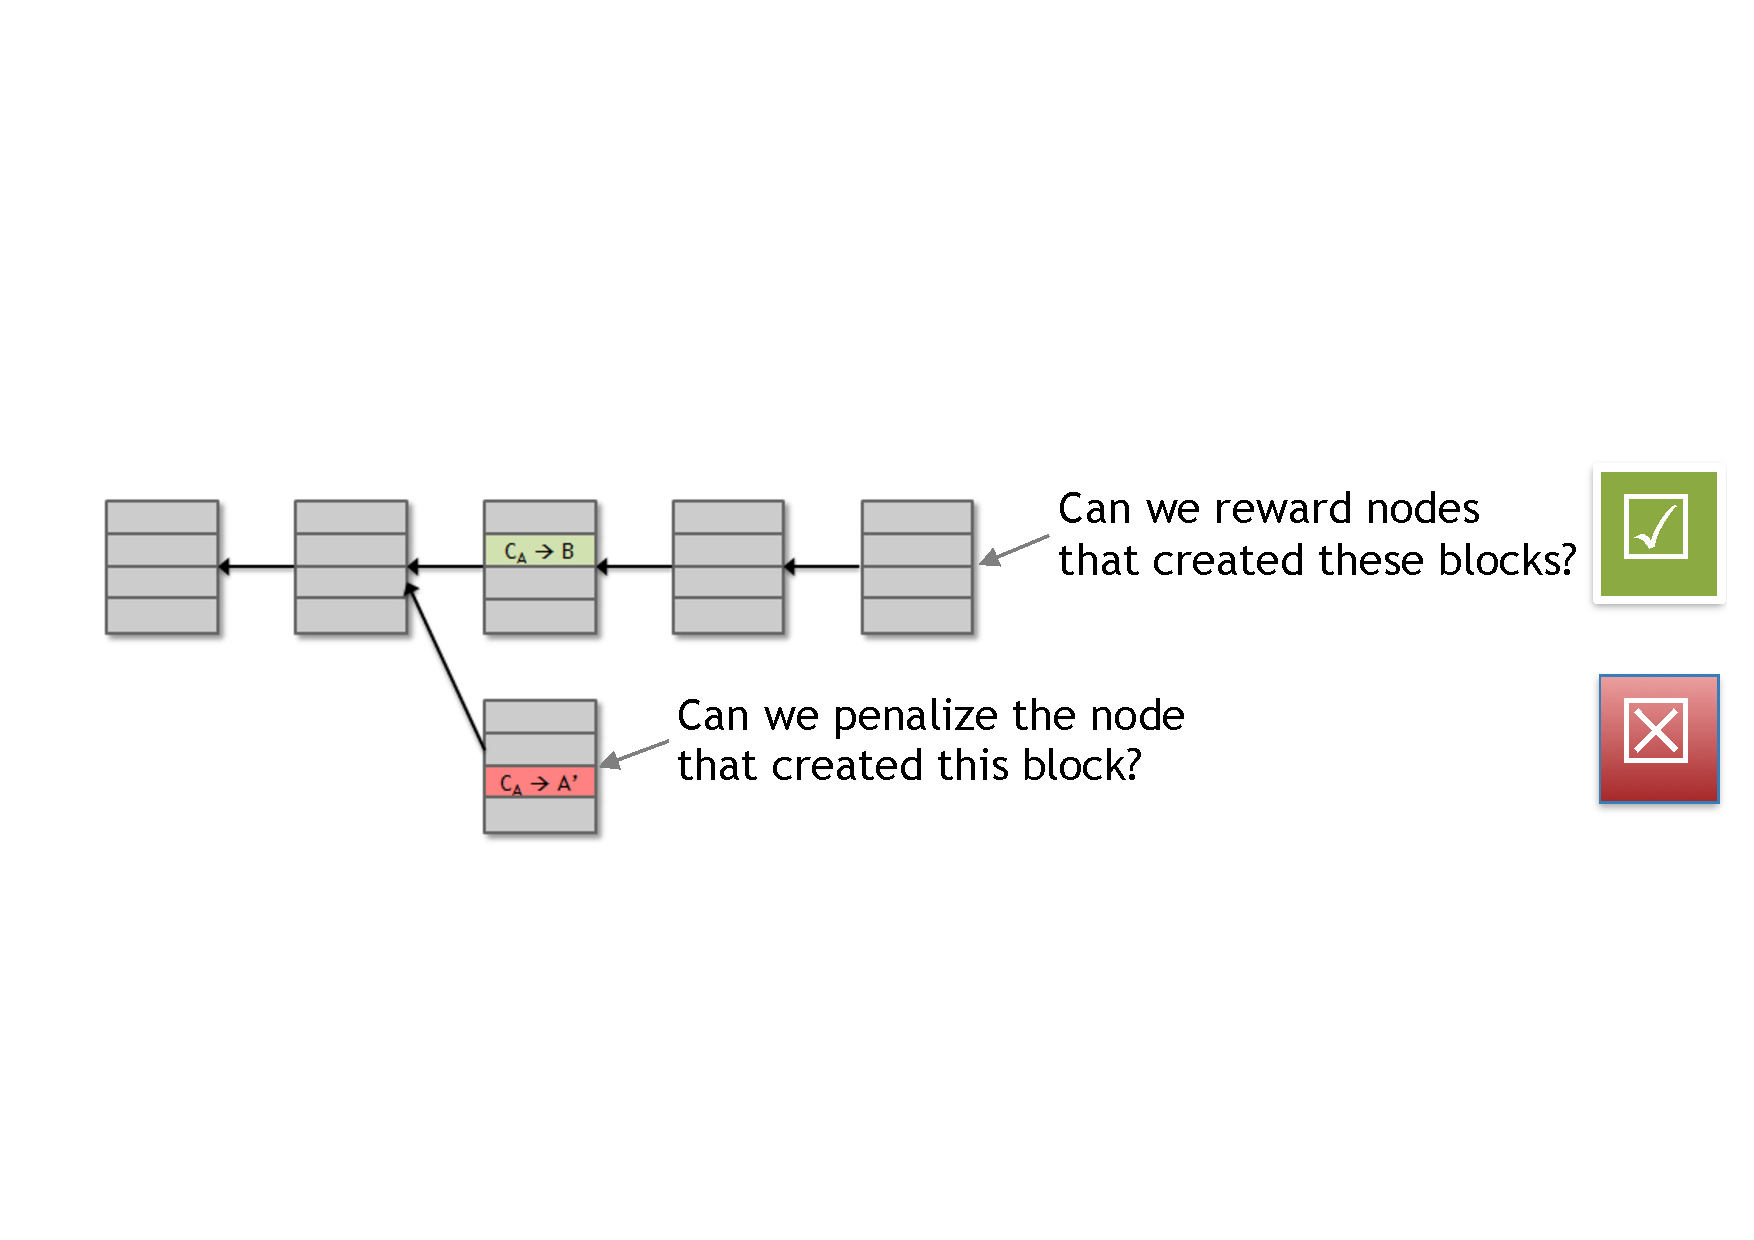
\includegraphics[width=\textwidth]{reward}

\BIL
\item Creator of block gets to
	\BI
	\item include special coin-creation transaction in the block
	\item choose recipient address of this transaction
	\EI
\item Value is fixed: currently 25 BTC, halves every 4 years
\item Block creator gets to “collect” the reward only if the block ends up on long-term consensus branch!
\EIL
	
\end{frame}

%-------------------------------------------------------------------------
\begin{frame}{Finite supply of Bitcoins}
	
\begin{columns}[T]
\begin{column}{0.55\textwidth}
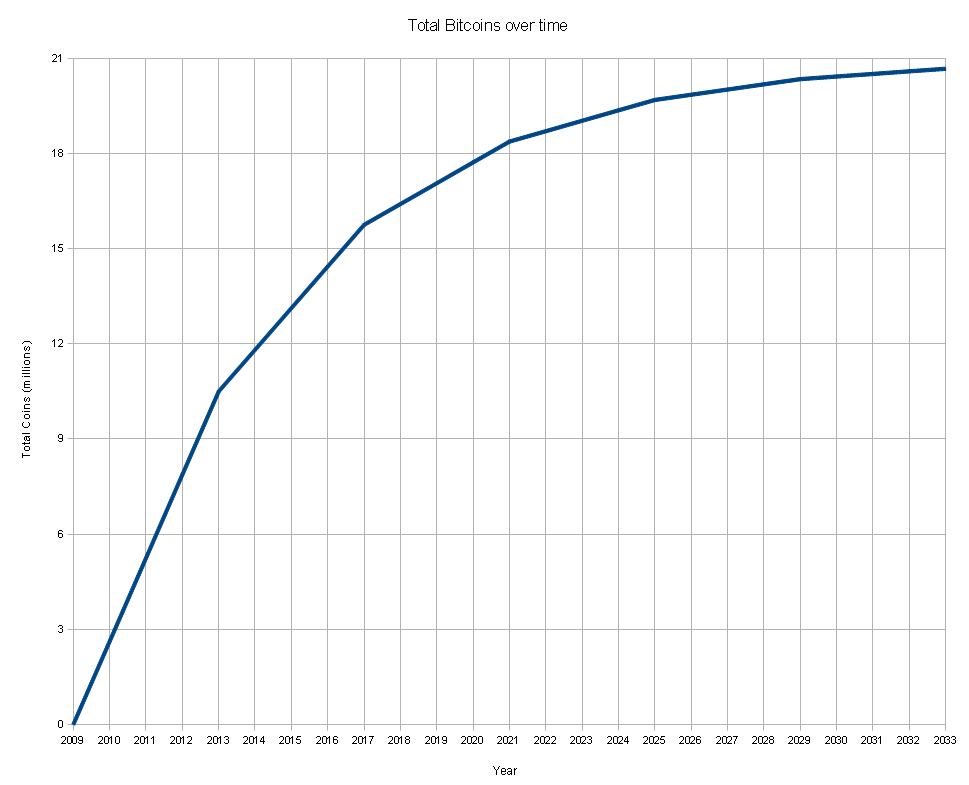
\includegraphics[width=\textwidth]{bitcoin.png}
\end{column}
\begin{column}{0.45\textwidth}
\BI
\item Total supply: 21 million
\item Block reward is how new Bitcoins are created
\item Runs out in 2140. No new bitcoins unless rules change
\EI
\end{column}
\end{columns}
\end{frame}

%-------------------------------------------------------------------------
\begin{frame}{Selecting the random node}

\BB{Problems}
\BI
\item How to pick a random node?
\item How to avoid a free-for-all due to rewards?
\item How to prevent Sybil attacks?
\EI

\BB{Proof-of-work}
\BIL
\item To approximate selecting a random node: 
	\BI
	\item select nodes in proportion to a resource that no one can monopolize (we hope)
	\EI
\item Equivalent views of proof of work
	\BI
	\item Select nodes in proportion to computing power
	\item Let nodes compete for right to create block
	\item Make it moderately hard to create new identities
	\EI
\EIL

\end{frame}

%-------------------------------------------------------------------------
\begin{frame}{Hash puzzles}
	
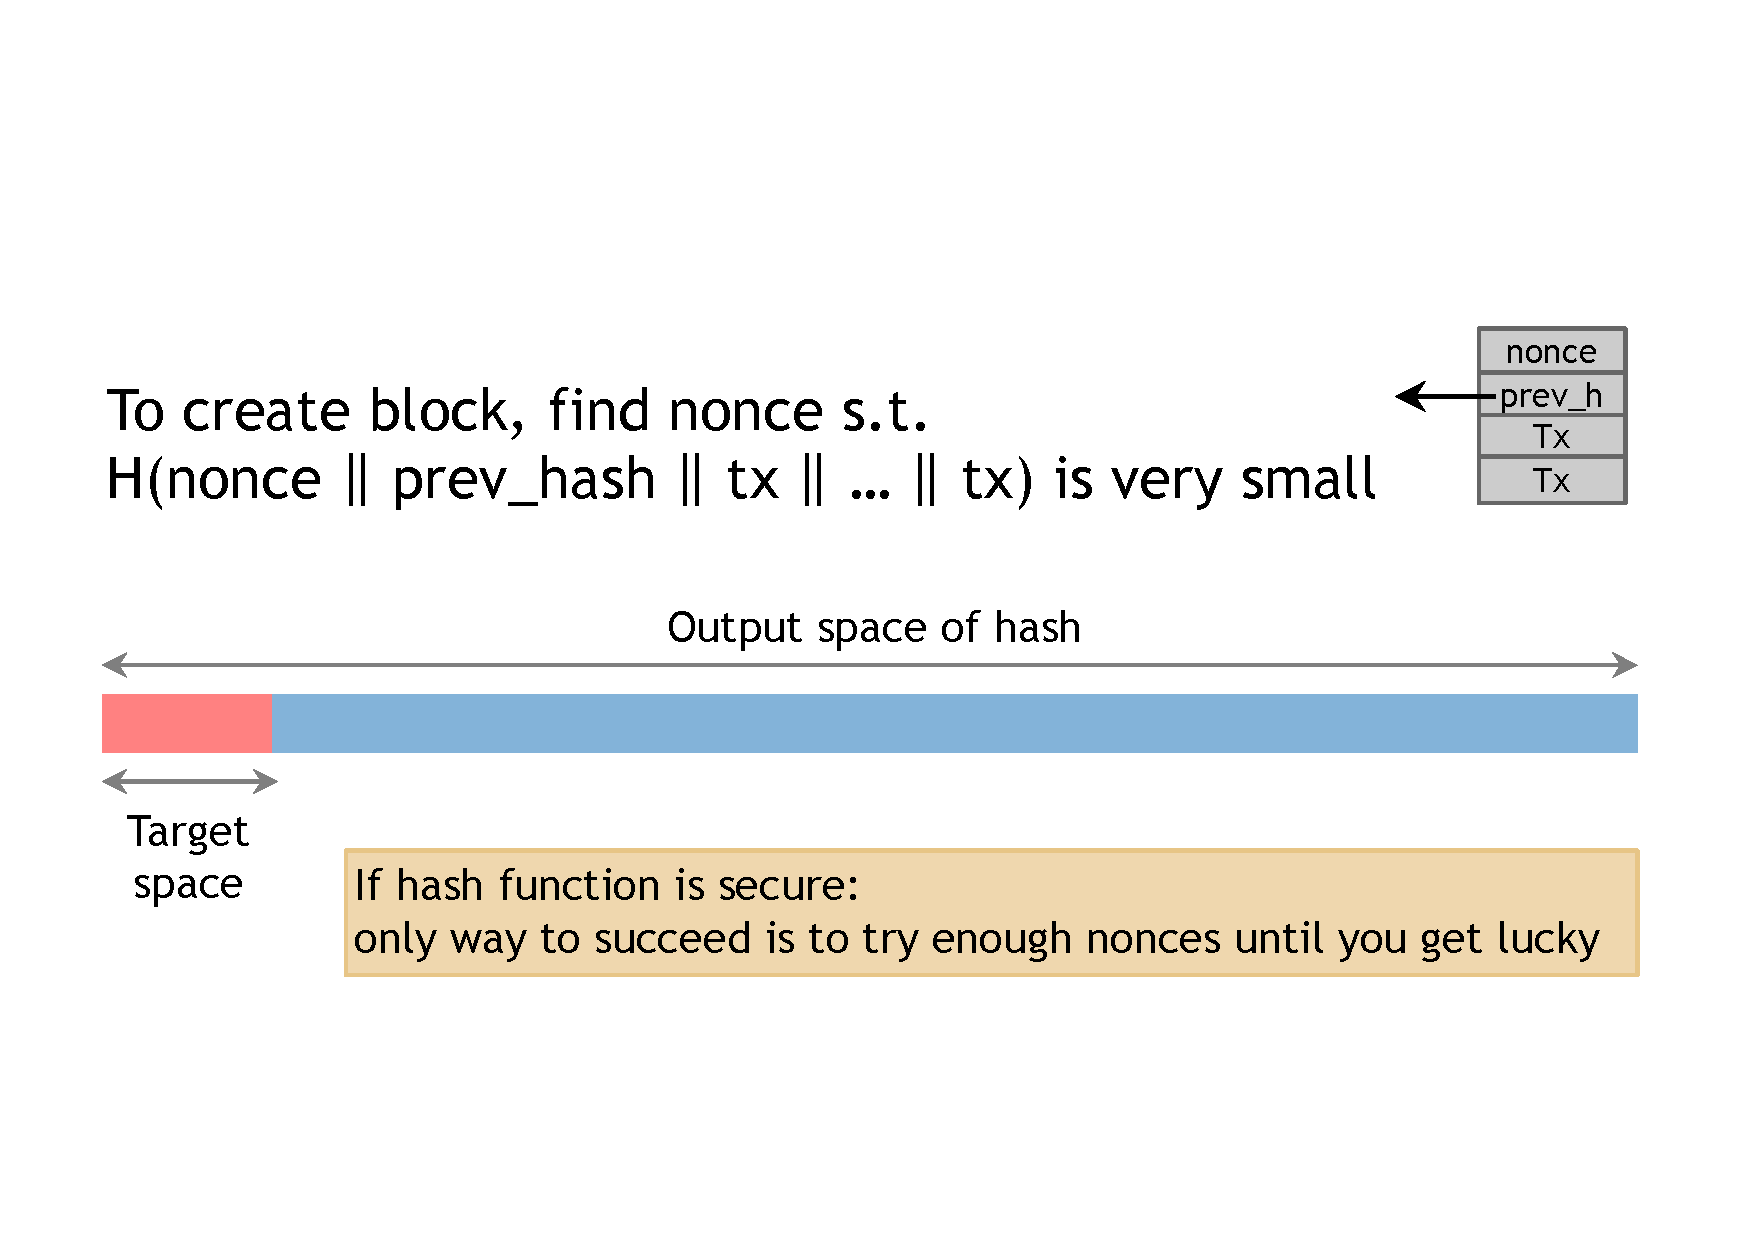
\includegraphics[width=\textwidth]{puzzle}
	
\end{frame}

%-------------------------------------------------------------------------
\begin{frame}{Proof-of-work properties}
	
\BB{Property 1: Difficult to compute}
\BI
\item As of Aug 2014: about $10^{20}$ hashes/block
\item Only some nodes bother to compete — miners
\EI

\BB{Property 2: Parameterizable cost}
\BI
\item Nodes automatically re-calculate the target every two weeks
\item  Goal: average time between blocks = 10 minutes
\EI

\BB{Property 3: Trivial to verify}
\BI
\item Nonce must be published as part of block
\item Other miners simply verify that
$H(\mathit{nonce} || \mathit{prev\_hash} || \mathit{tx} || \ldots || \mathit{tx}) < \mathit{target}$
\EI


\end{frame}

%-------------------------------------------------------------------------
\begin{frame}{Solving hash puzzles is probabilistic}
	
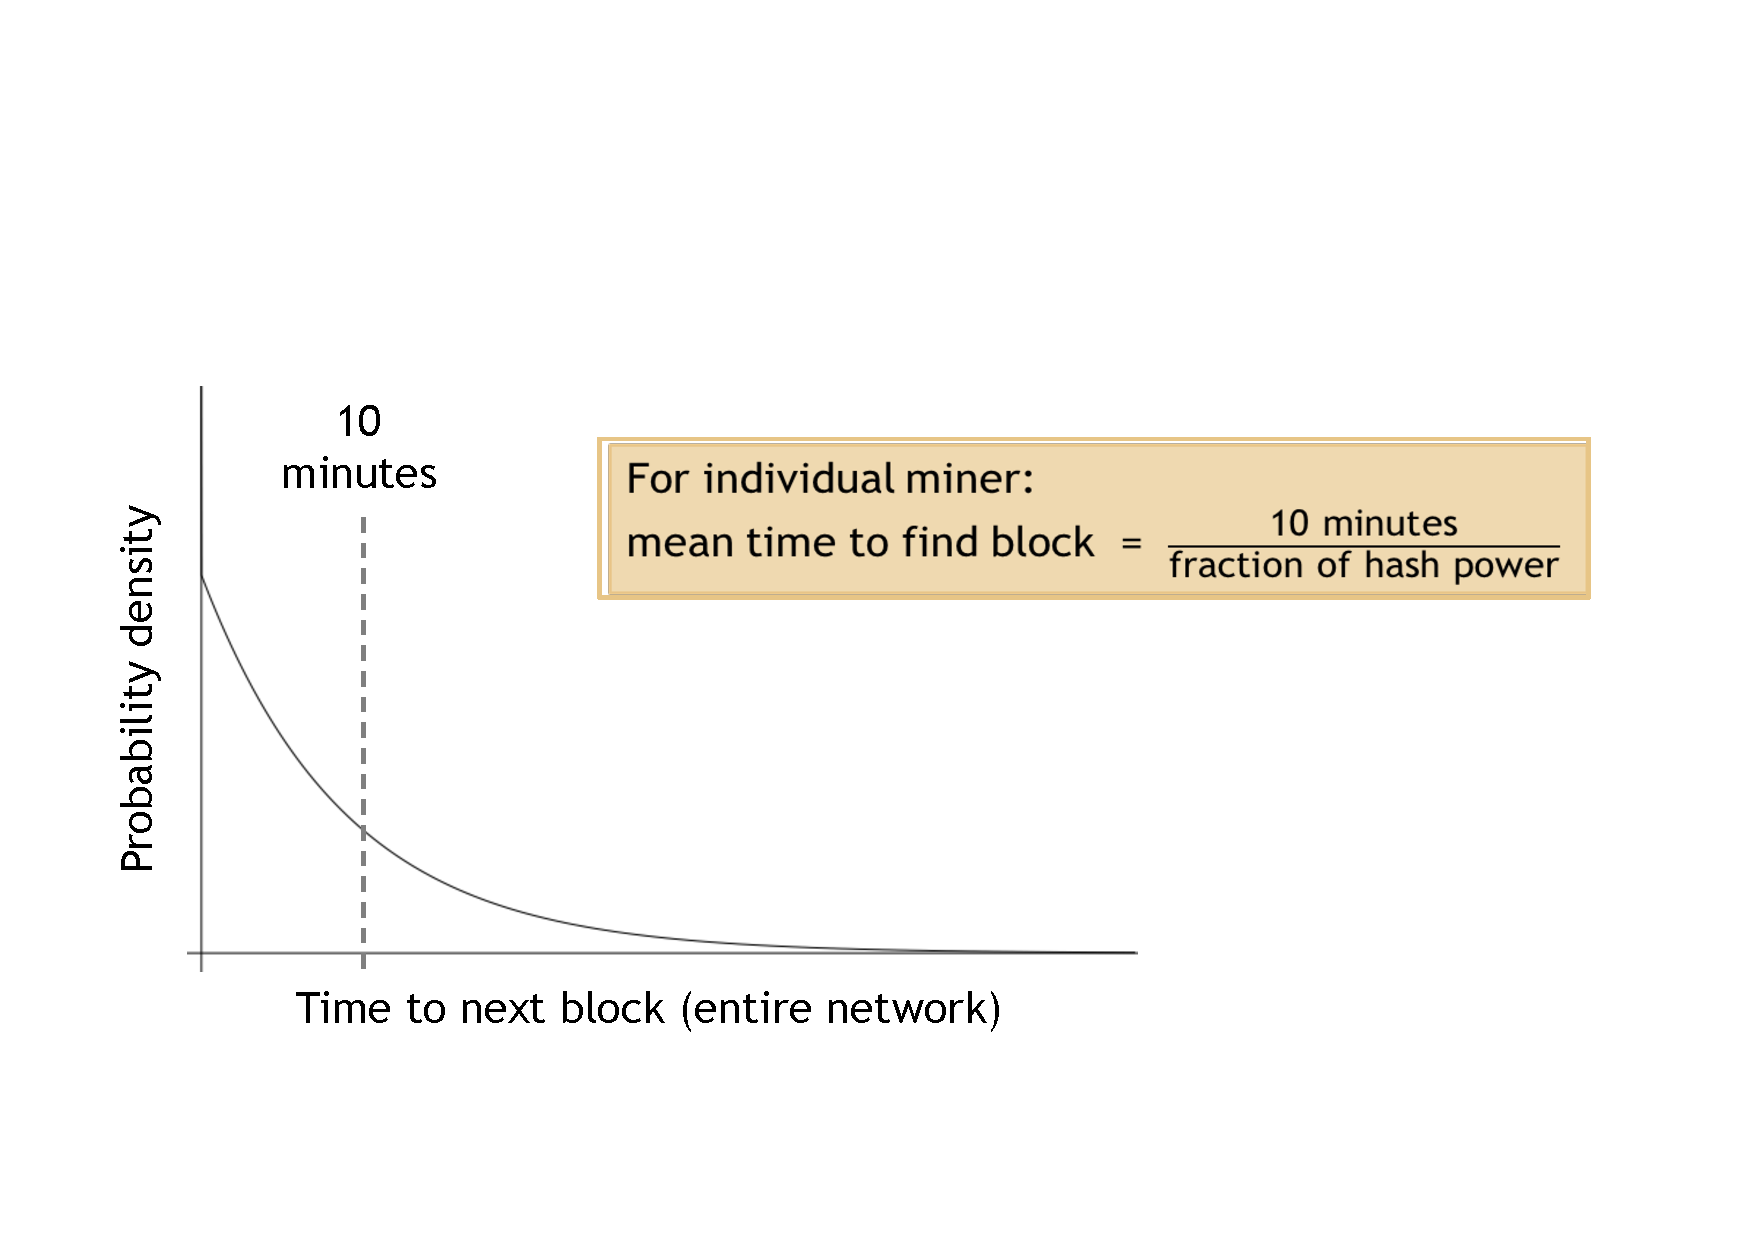
\includegraphics[width=\textwidth]{solving}

\end{frame}

%-------------------------------------------------------------------------
\begin{frame}{51\% Attacks}
	
\BB{Key security assumption}
\BI
\item Attacks infeasible if majority of miners weighted by hash power follow the protocol
\EI

\BB{What can a “51\% attacker” do?}
\BI
\item Steal coins from existing address? \onslide<2-6|handout:1>{NO}
\item Suppress some transactions 
	\BI
	\item From the blockchain? \onslide<3-6|handout:1>{YES}
	\item From the P2P network \onslide<4-6|handout:1>{NO}
	\EI
\item Change the block reward? \onslide<5-6|handout:1>{NO}
\item Destroy confidence in Bitcoin? \onslide<6|handout:1>{YES!!!}	
\EI 

\end{frame}

%%%%%%%%%%%%%%%%%%%%%%%%%%%%%%%%%
\section{Conclusions}
%%%%%%%%%%%%%%%%%%%%%%%%%%%%%%%%%

\begin{frame}{Limits for Bitcoin}

\BB{Hard-coded limits for BitCoin}

\BI
\item 10 min. average creation time per block
\item 1M bytes in a block
\item 20,000 signature operations per block
\item 21M total Bitcoins maximum
\item 50,25,12.5... Bitcoin mining reward
\EI

\BB{Throughput limits in Bitcoin}

\BI
\item 1 Mbytes/block every 10 minutes
\item $>250$ bytes/transaction
\item 7 transactions/sec 
\item Compare to:
	\BI
	\item VISA: 2,000-10,000 transactions/sec
	\item PayPal: 50-100 transaction/sec
	\EI
\EI
\end{frame}

\begin{frame}{Extensions of BitCoin}

\BB{Beyond money}

\BIL
\item Scripting
	\BI
	\item 2-out-3 signatures
	\EI
\item Distributed Execution of derivatives-contracts-as-Programs
\item Altcoins
\EIL
\end{frame}



%-------------------------------------------------------------------------
\begin{RMFrame}

\BI
\item \bibentry{bitcoin}
\item In this presentation: Chapters 1-3 (77 pages)
\item Warning: 300+ pages
\EI

\end{RMFrame}


\end{document}




